\documentclass[11pt]{article}

\usepackage{amsmath}
\usepackage{graphicx}
\usepackage{subcaption}

\newcommand{\numpy}{{\tt numpy}}    % tt font for numpy

\topmargin -.5in
\textheight 9in
\oddsidemargin -.25in
\evensidemargin -.25in
\textwidth 7in

\begin{document}

% ========== Edit your name here
\author{Aobo Yang (ay6gv)}
\title{CS6316: HW4}
\maketitle

\medskip

% ========== Begin answering questions here
\begin{enumerate}

\item
Neural Network Playground

1.1
\medskip

Frigure \ref{fig:circle} is the screenshot for dataset Circle. The features chosen are $x_1^2$ and $x_2^2$. The best test loss is $0.000$ which is achieved after $1037$ iterations. The features work because the function of a circle is $x_1^2 + x_2^2 = c$.

\begin{figure}[!h]
  \centering
  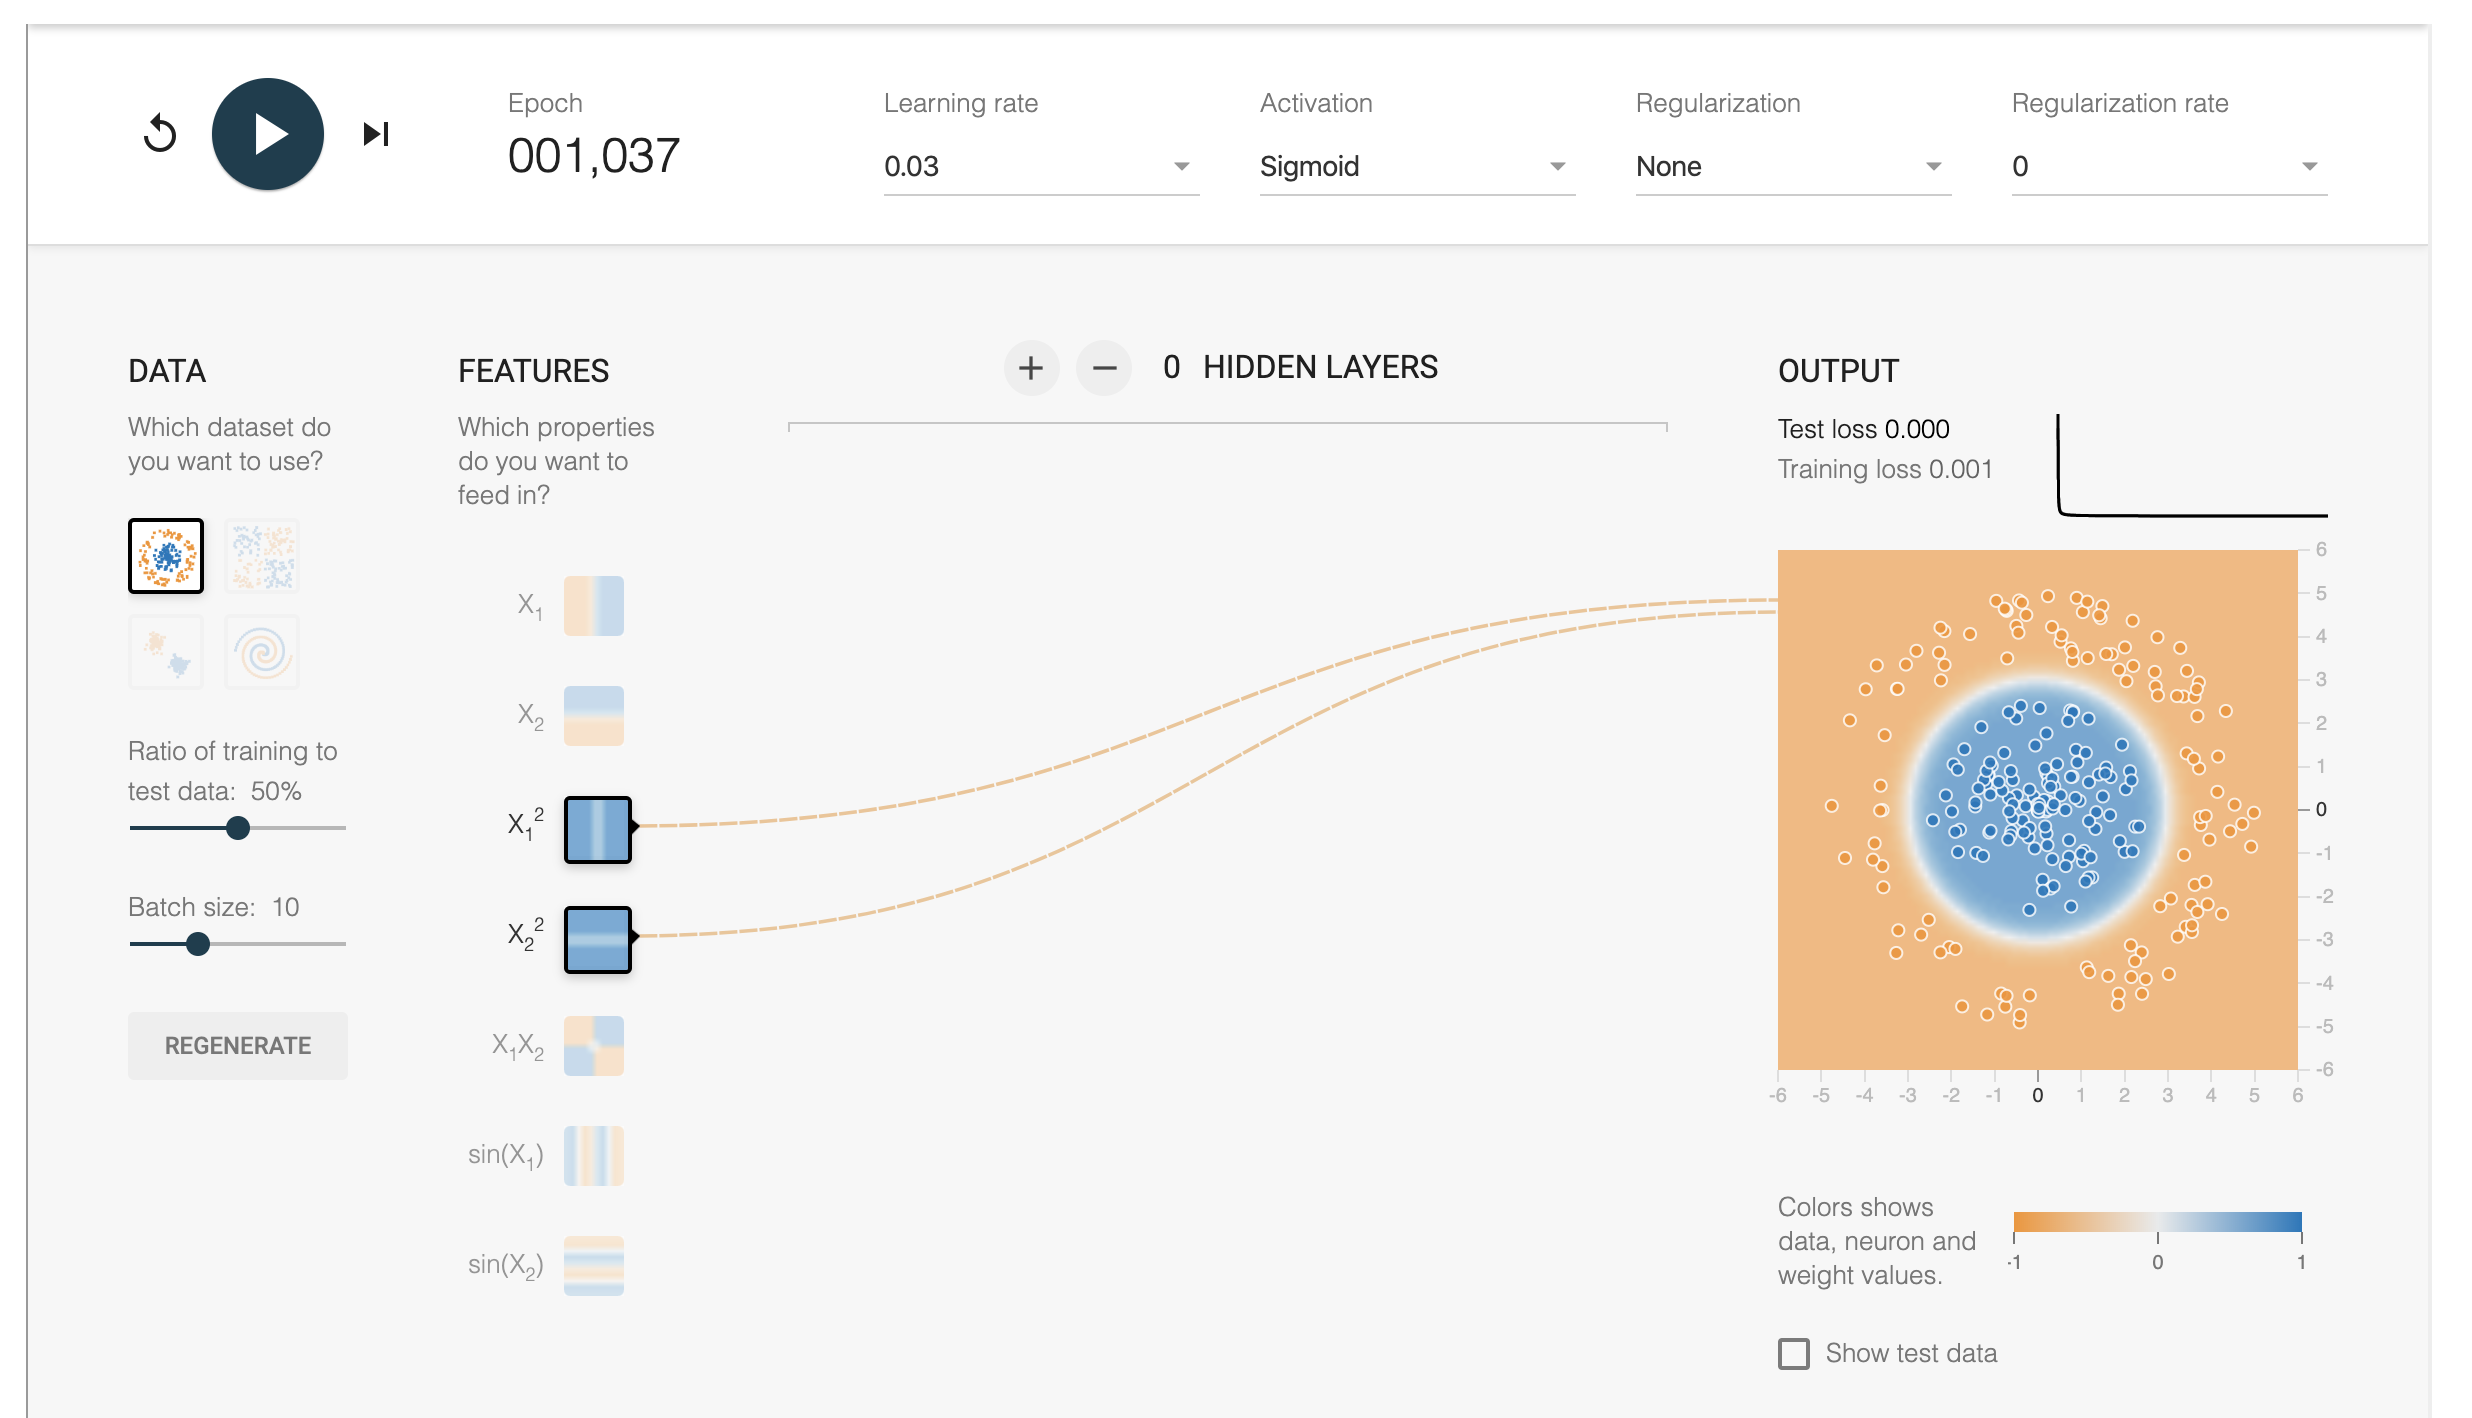
\includegraphics[width=\linewidth]{figures/1_1/circle.png}
  \caption{Circle}
  \label{fig:circle}
\end{figure}


Frigure \ref{fig:exclusive_or} is the screenshot for dataset Exclusive. The only feature chosen is $x_1x_2$. The best test loss is $0.000$ which is achieved after $1633$ iterations. The features work because the data of exlusive or is labeled based on if $x_1x_2$ is postive or negative.

\begin{figure}[!h]
  \centering
  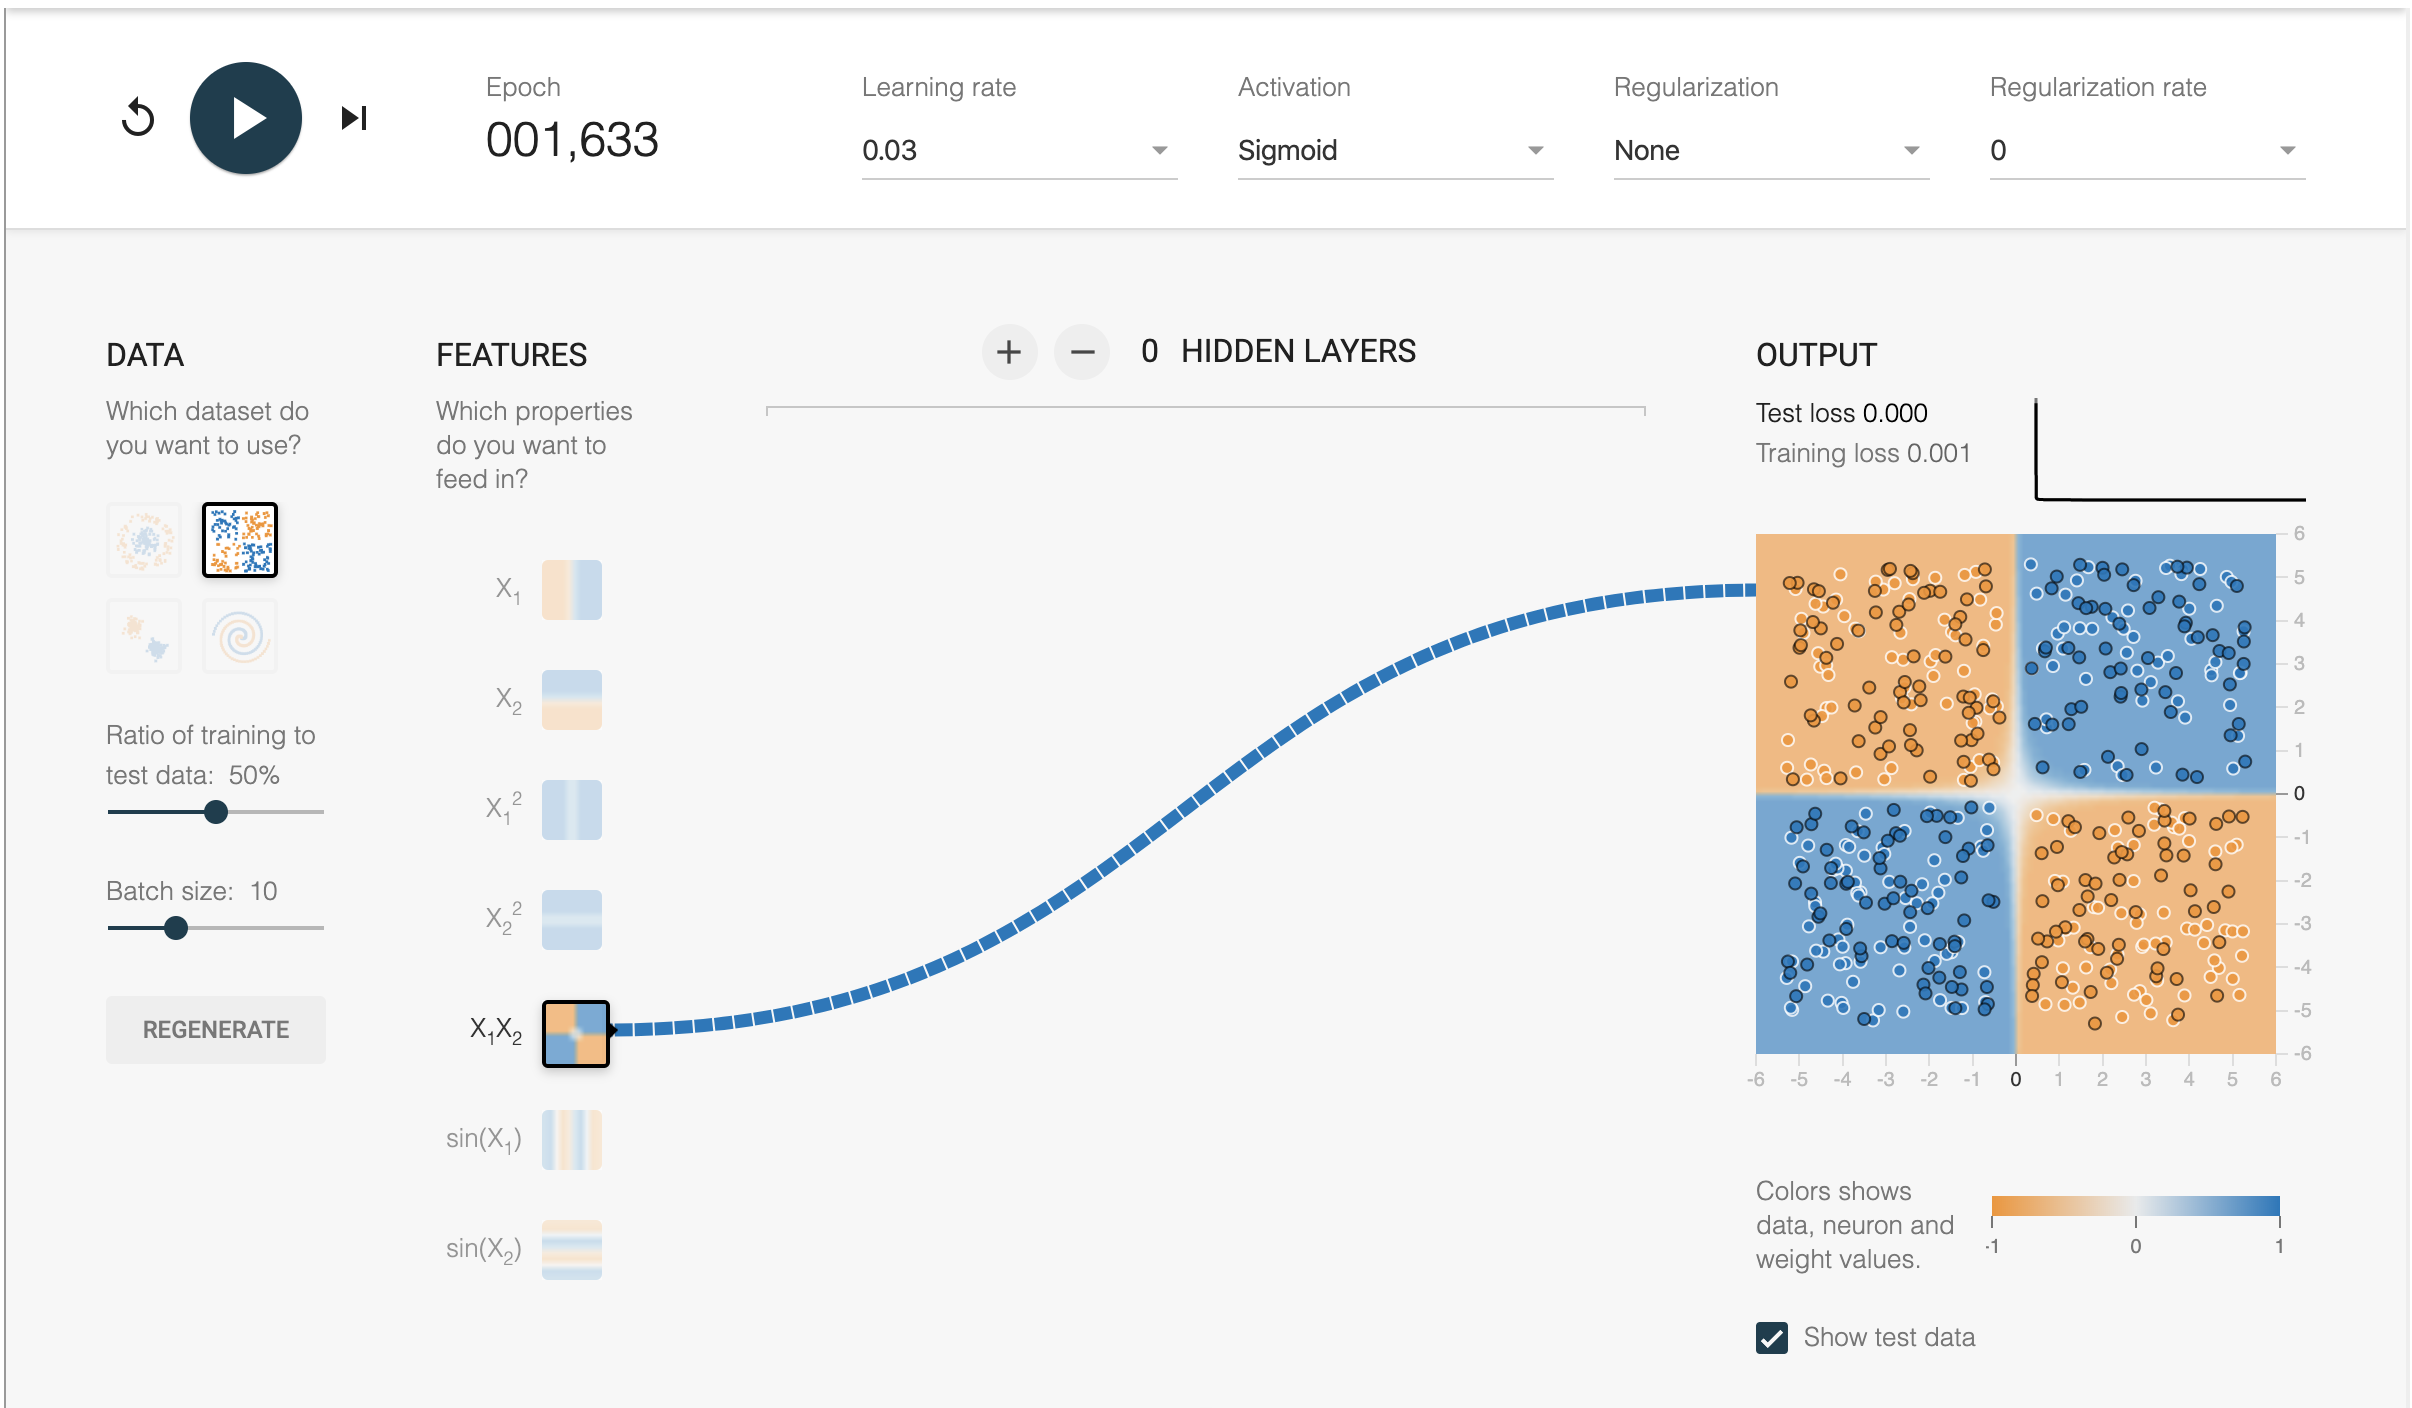
\includegraphics[width=\linewidth]{figures/1_1/exclusive_or.png}
  \caption{Exclusive}
  \label{fig:exclusive_or}
\end{figure}

Frigure \ref{fig:gaussian} is the screenshot for dataset Gaussian. The features chosen are $x_1$ and $x_2$. The best test loss is $0.000$ which is achieved after $158$ iterations. The features work because the the decision boundary based on if $x_1 + x_2$ is positive or negative can separate the well separate the data.

\begin{figure}[!h]
  \centering
  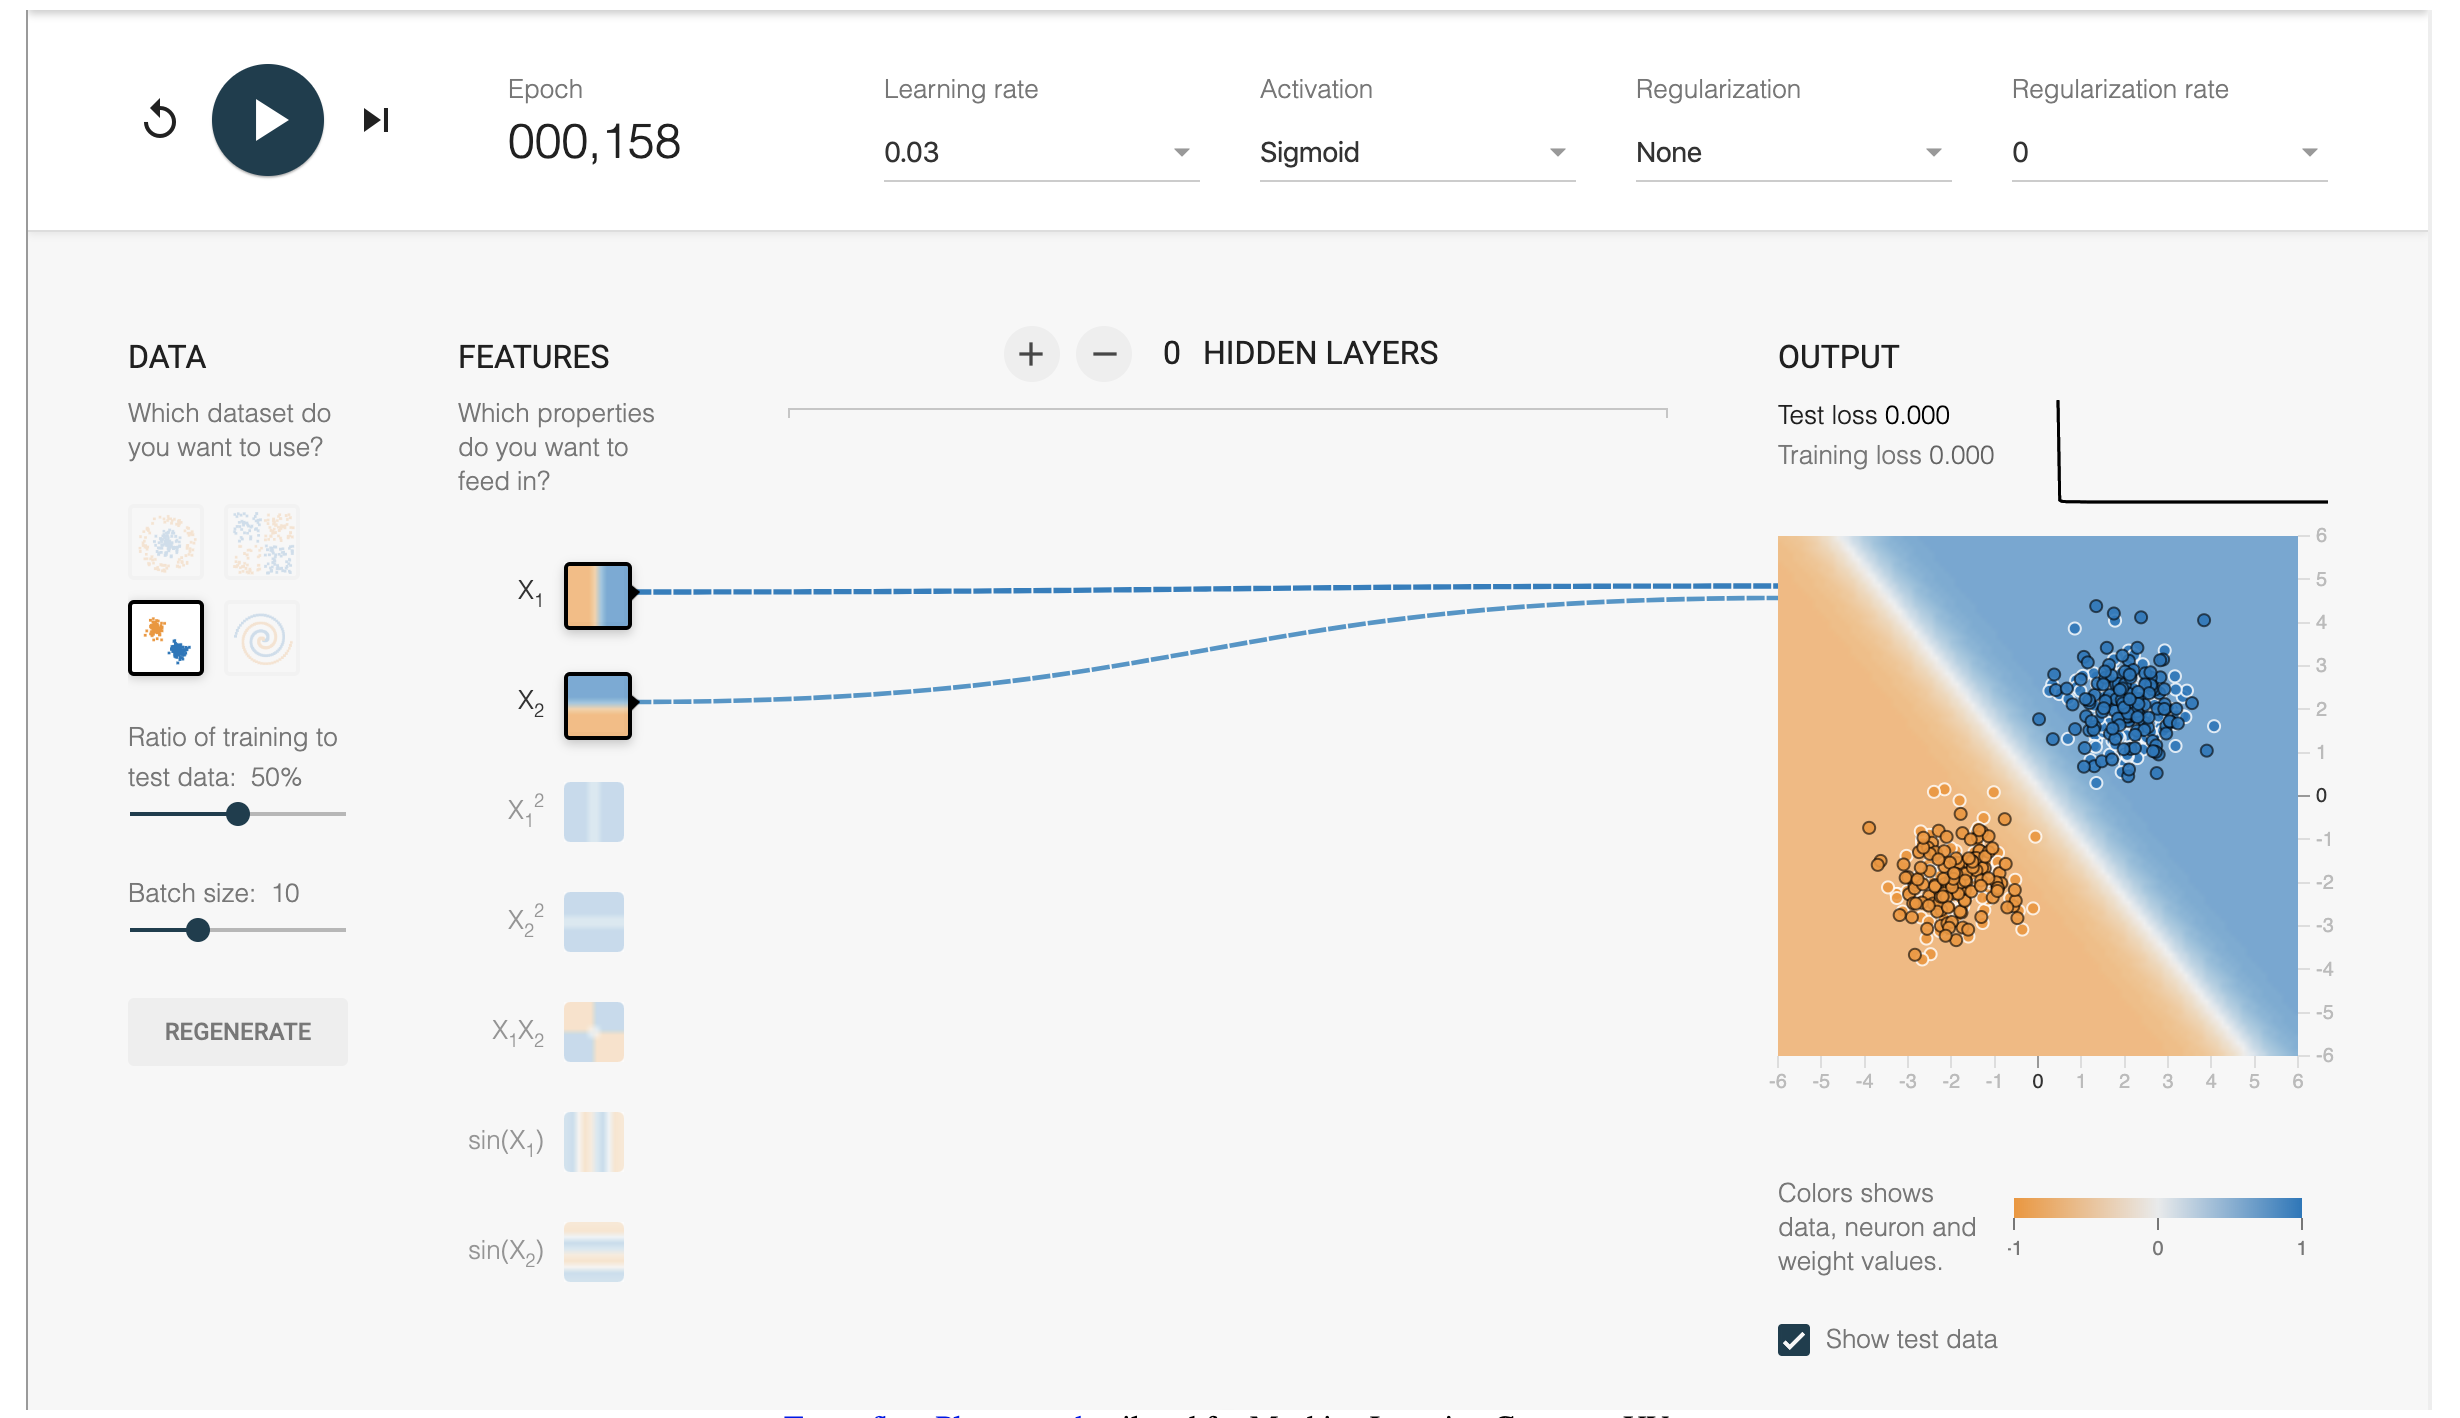
\includegraphics[width=\linewidth]{figures/1_1/gaussian.png}
  \caption{Gaussian}
  \label{fig:gaussian}
\end{figure}


Frigure \ref{fig:spiral} is the screenshot for dataset Spiral. The features chosen are $x_1$, $x_2$ and $x_1x_2$. The best test loss is $0.464$ which is achieved after $230$ iterations. The features are not enough to well separate the data.

\begin{figure}[!h]
  \centering
  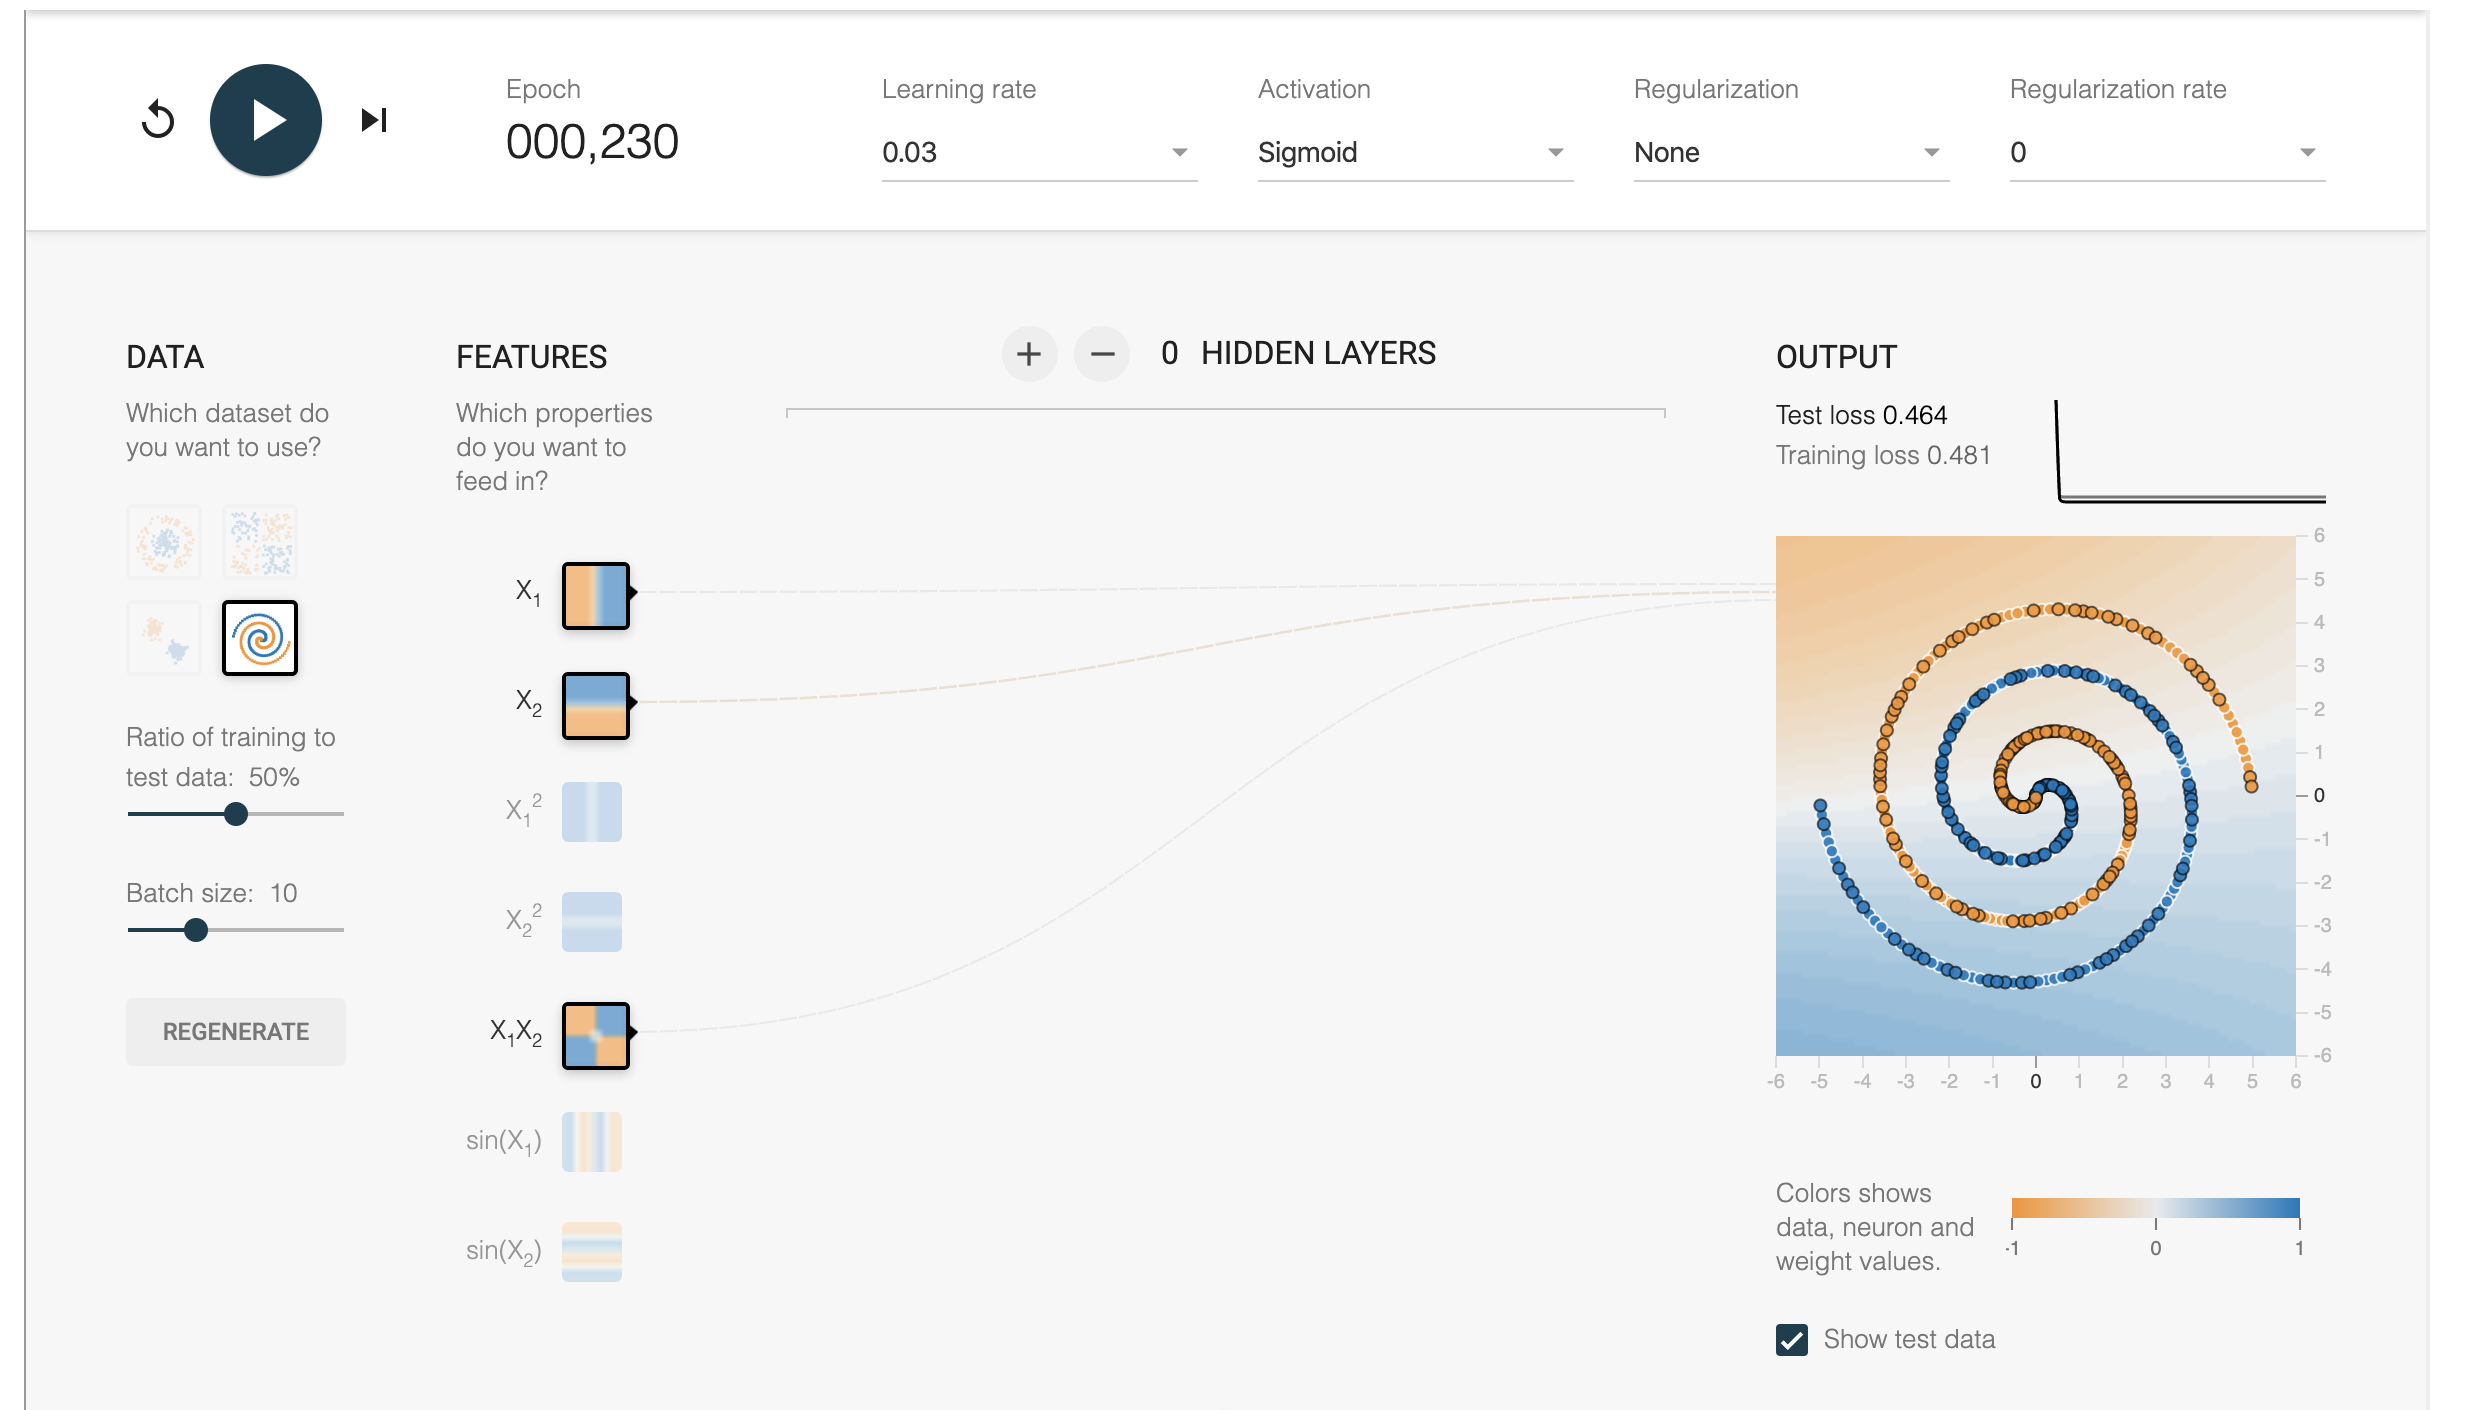
\includegraphics[width=\linewidth]{figures/1_1/spiral.png}
  \caption{Spiral}
  \label{fig:spiral}
\end{figure}

1.2
\medskip

Task A
\medskip

For circle data, the best loss of each regularization after $500$ iterations is shown in table below. The result of L1 is shown in Firgure \ref{fig:circle_reg}. As we can see, the different regularizations do not really make any differences to the test loss. I choose L1 in the report. Under this configuration, the model sucessfully can recognize the importance of $x_1^2$ and $x_2^2$ as shown in the screenshot, so it works.

\begin{center}
  \begin{tabular}{ |c|c|c|c| }
   \hline
    No regularization & L1 regularized (0.003) & L2 regularized (0.003) \\
    0.001 & 0.001 & 0.001 \\
    \hline
  \end{tabular}
\end{center}


\begin{figure}[!h]
  \centering
  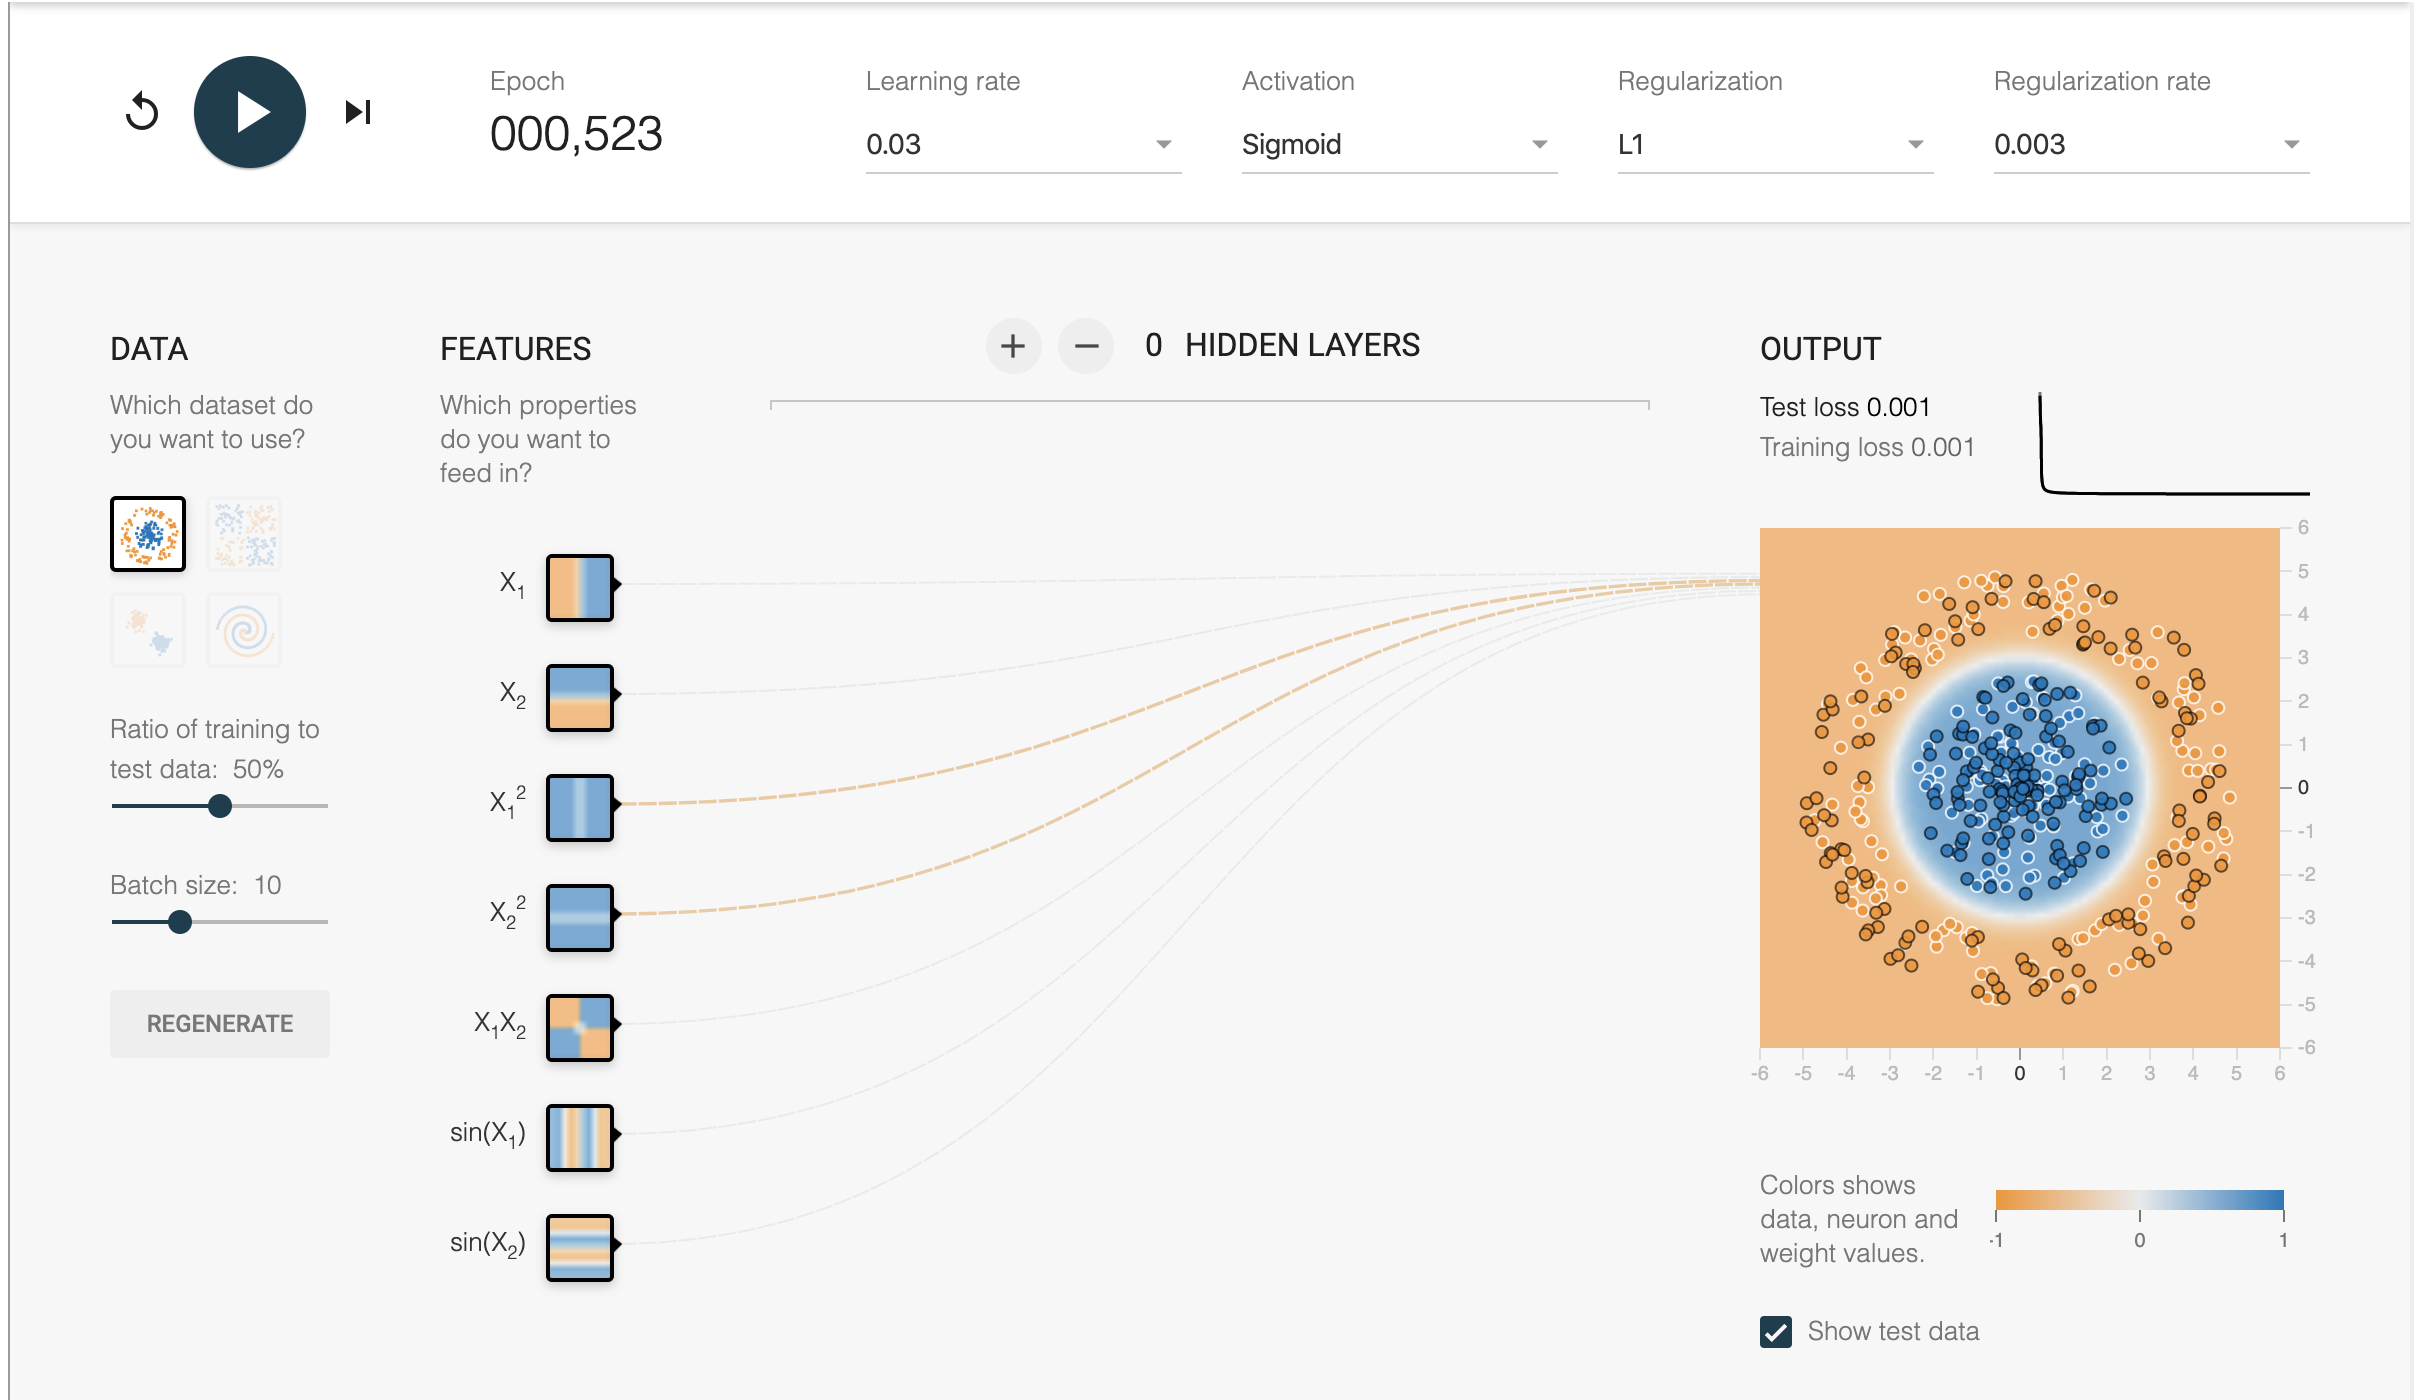
\includegraphics[width=\linewidth]{figures/1_2/circle.png}
  \caption{Circle Regularized}
  \label{fig:circle_reg}
\end{figure}

For exclusive or data, the best loss of each regularization after $250$ iterations is shown in table below. The result of L1 is shown in Firgure \ref{fig:exclusive_or_reg}. This configuration works better because exclusive or label is only decided by $x_1x_2$ and all other features are unrelated. As shown in the screenshot, the L1 regularization successfully help to find the right feature.

\begin{center}
  \begin{tabular}{ |c|c|c|c| }
   \hline
    No regularization & L1 regularized (0.003) & L2 regularized (0.001) \\
    0.013 & 0.008 & 0.013 \\
    \hline
  \end{tabular}
\end{center}


\begin{figure}[!h]
  \centering
  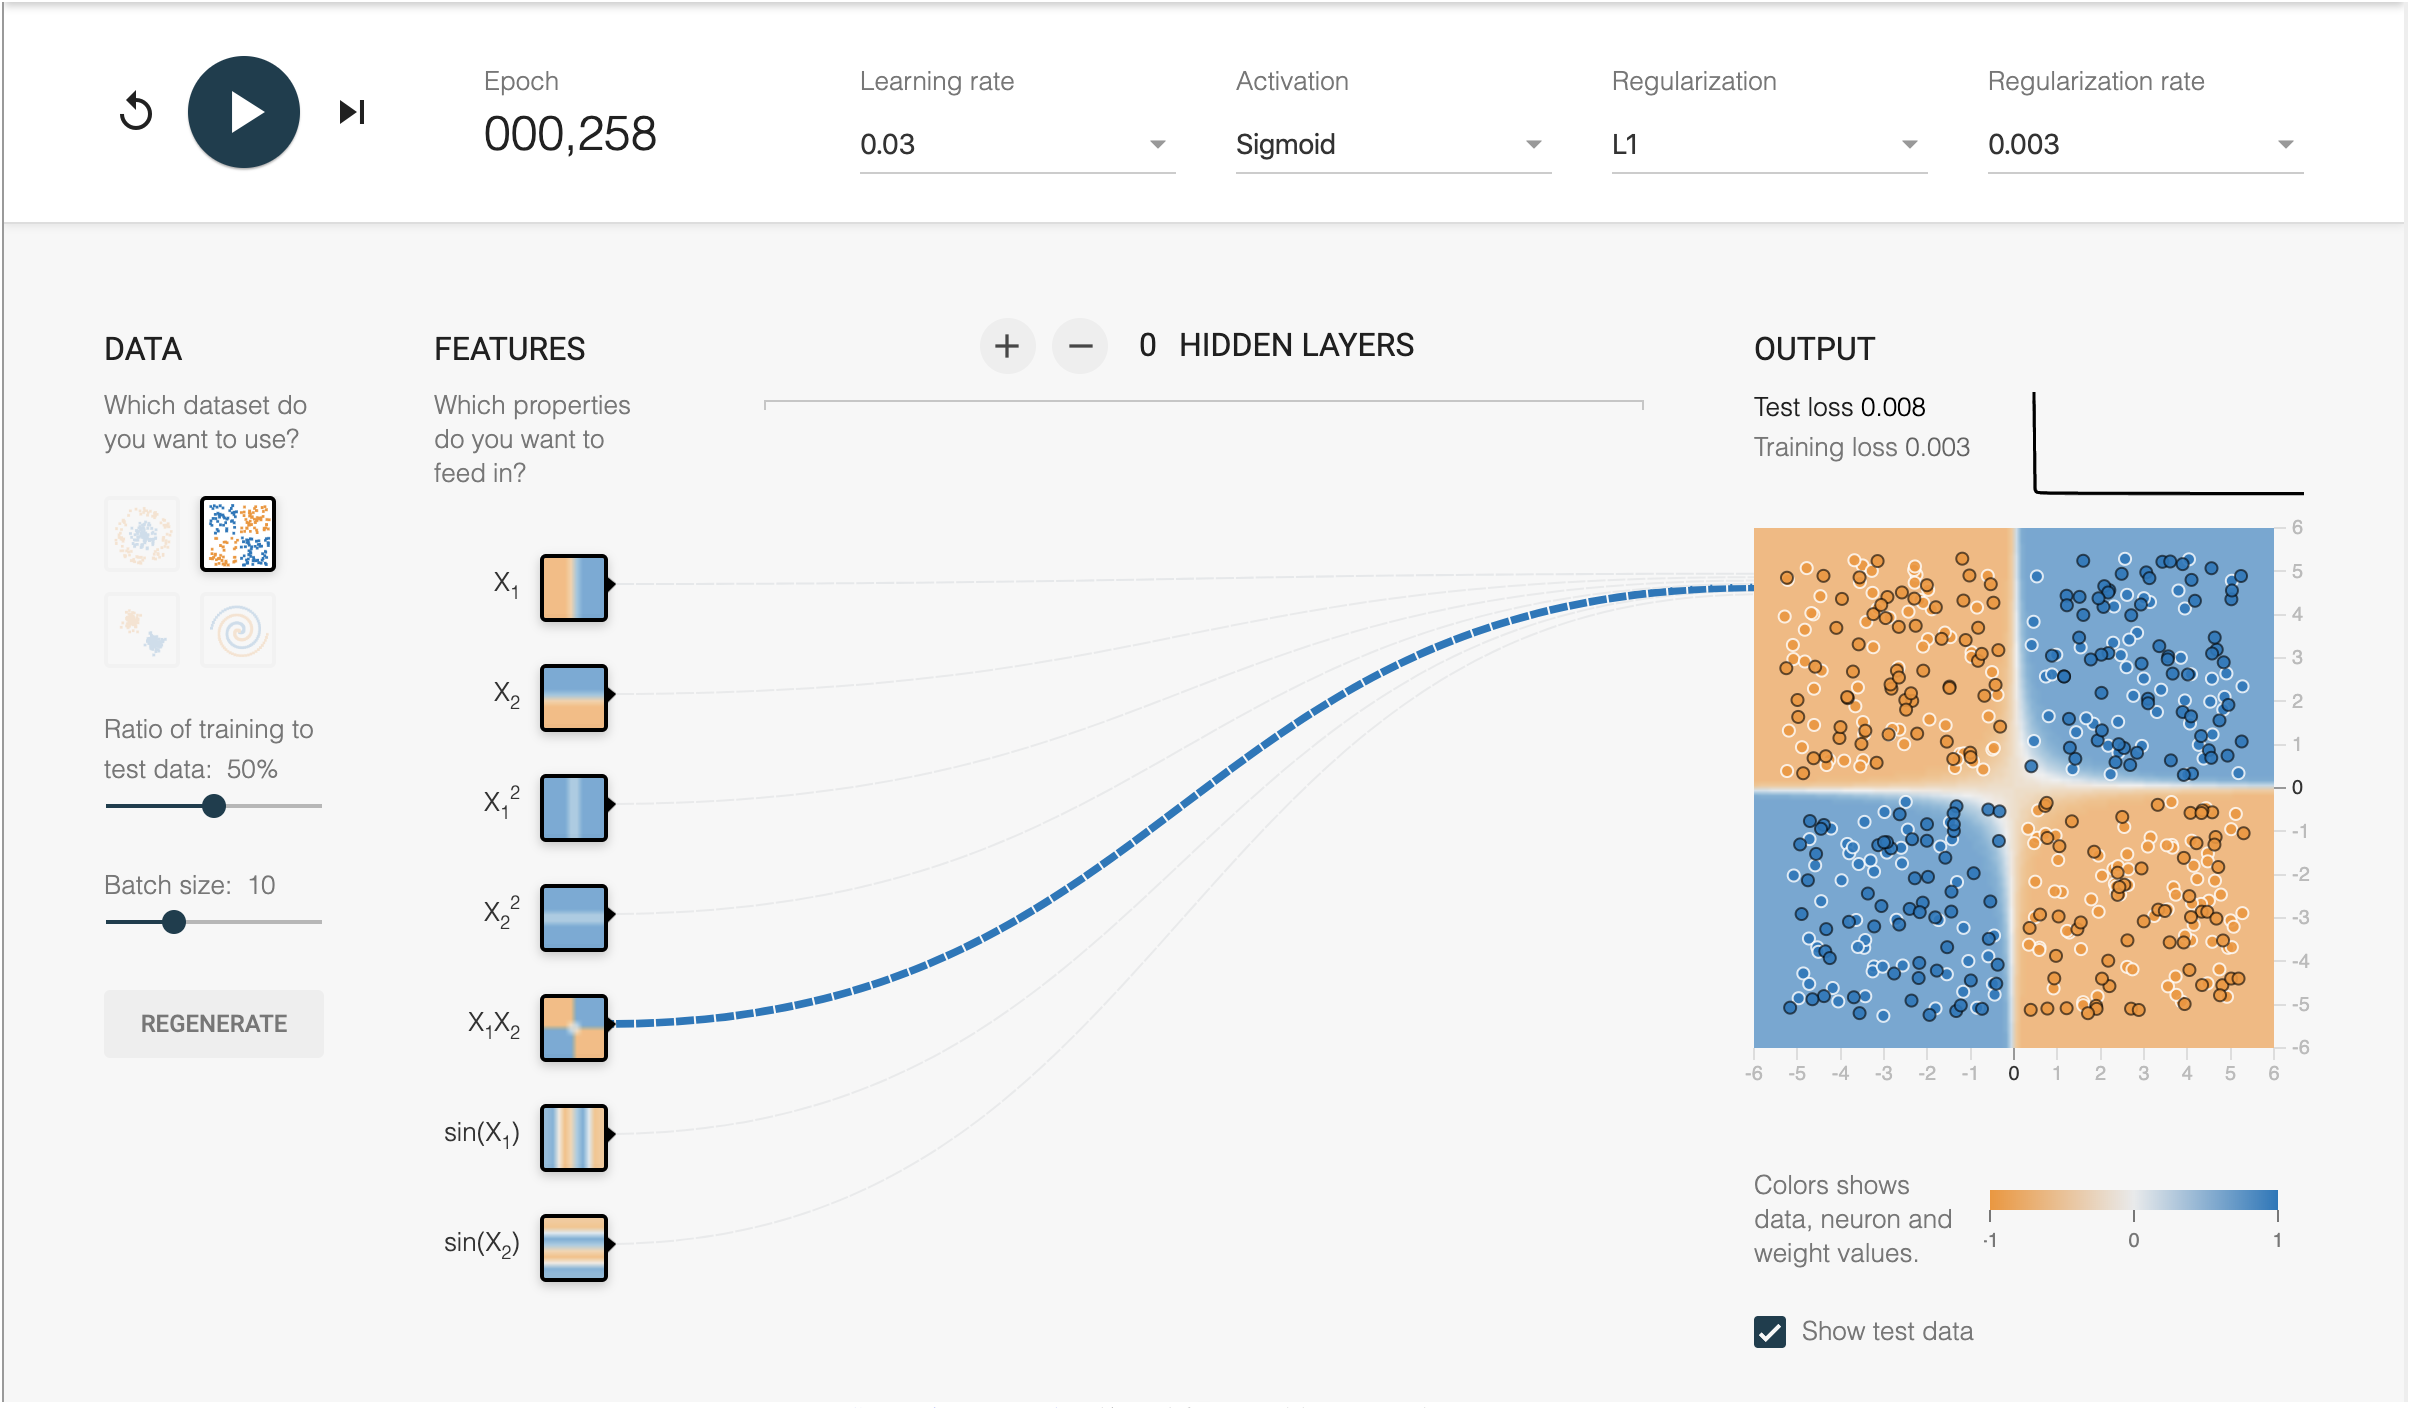
\includegraphics[width=\linewidth]{figures/1_2/exclusive_or.png}
  \caption{Exclusive Or Regularized}
  \label{fig:exclusive_or_reg}
\end{figure}


For gaussian data, the best loss of each regularization after $200$ iterations is shown in table below. The result of No regularization is shown in Firgure \ref{fig:gaussian_reg}. Because the data distribution of this set is concentrated and quite easy to separate, many different boundaries can work. Therefore, although regularizations can make the boundary looks more balanced and smooth, they have no advantages in test loss. The no regularization one I choose may be a little overfitted, but it indeed perfectly separate the testing data.

\begin{center}
  \begin{tabular}{ |c|c|c|c| }
   \hline
    No regularization & L1 regularized (0.001) & L2 regularized (0.001) \\
    0.000 & 0.000 & 0.001 \\
    \hline
  \end{tabular}
\end{center}


\begin{figure}[!h]
  \centering
  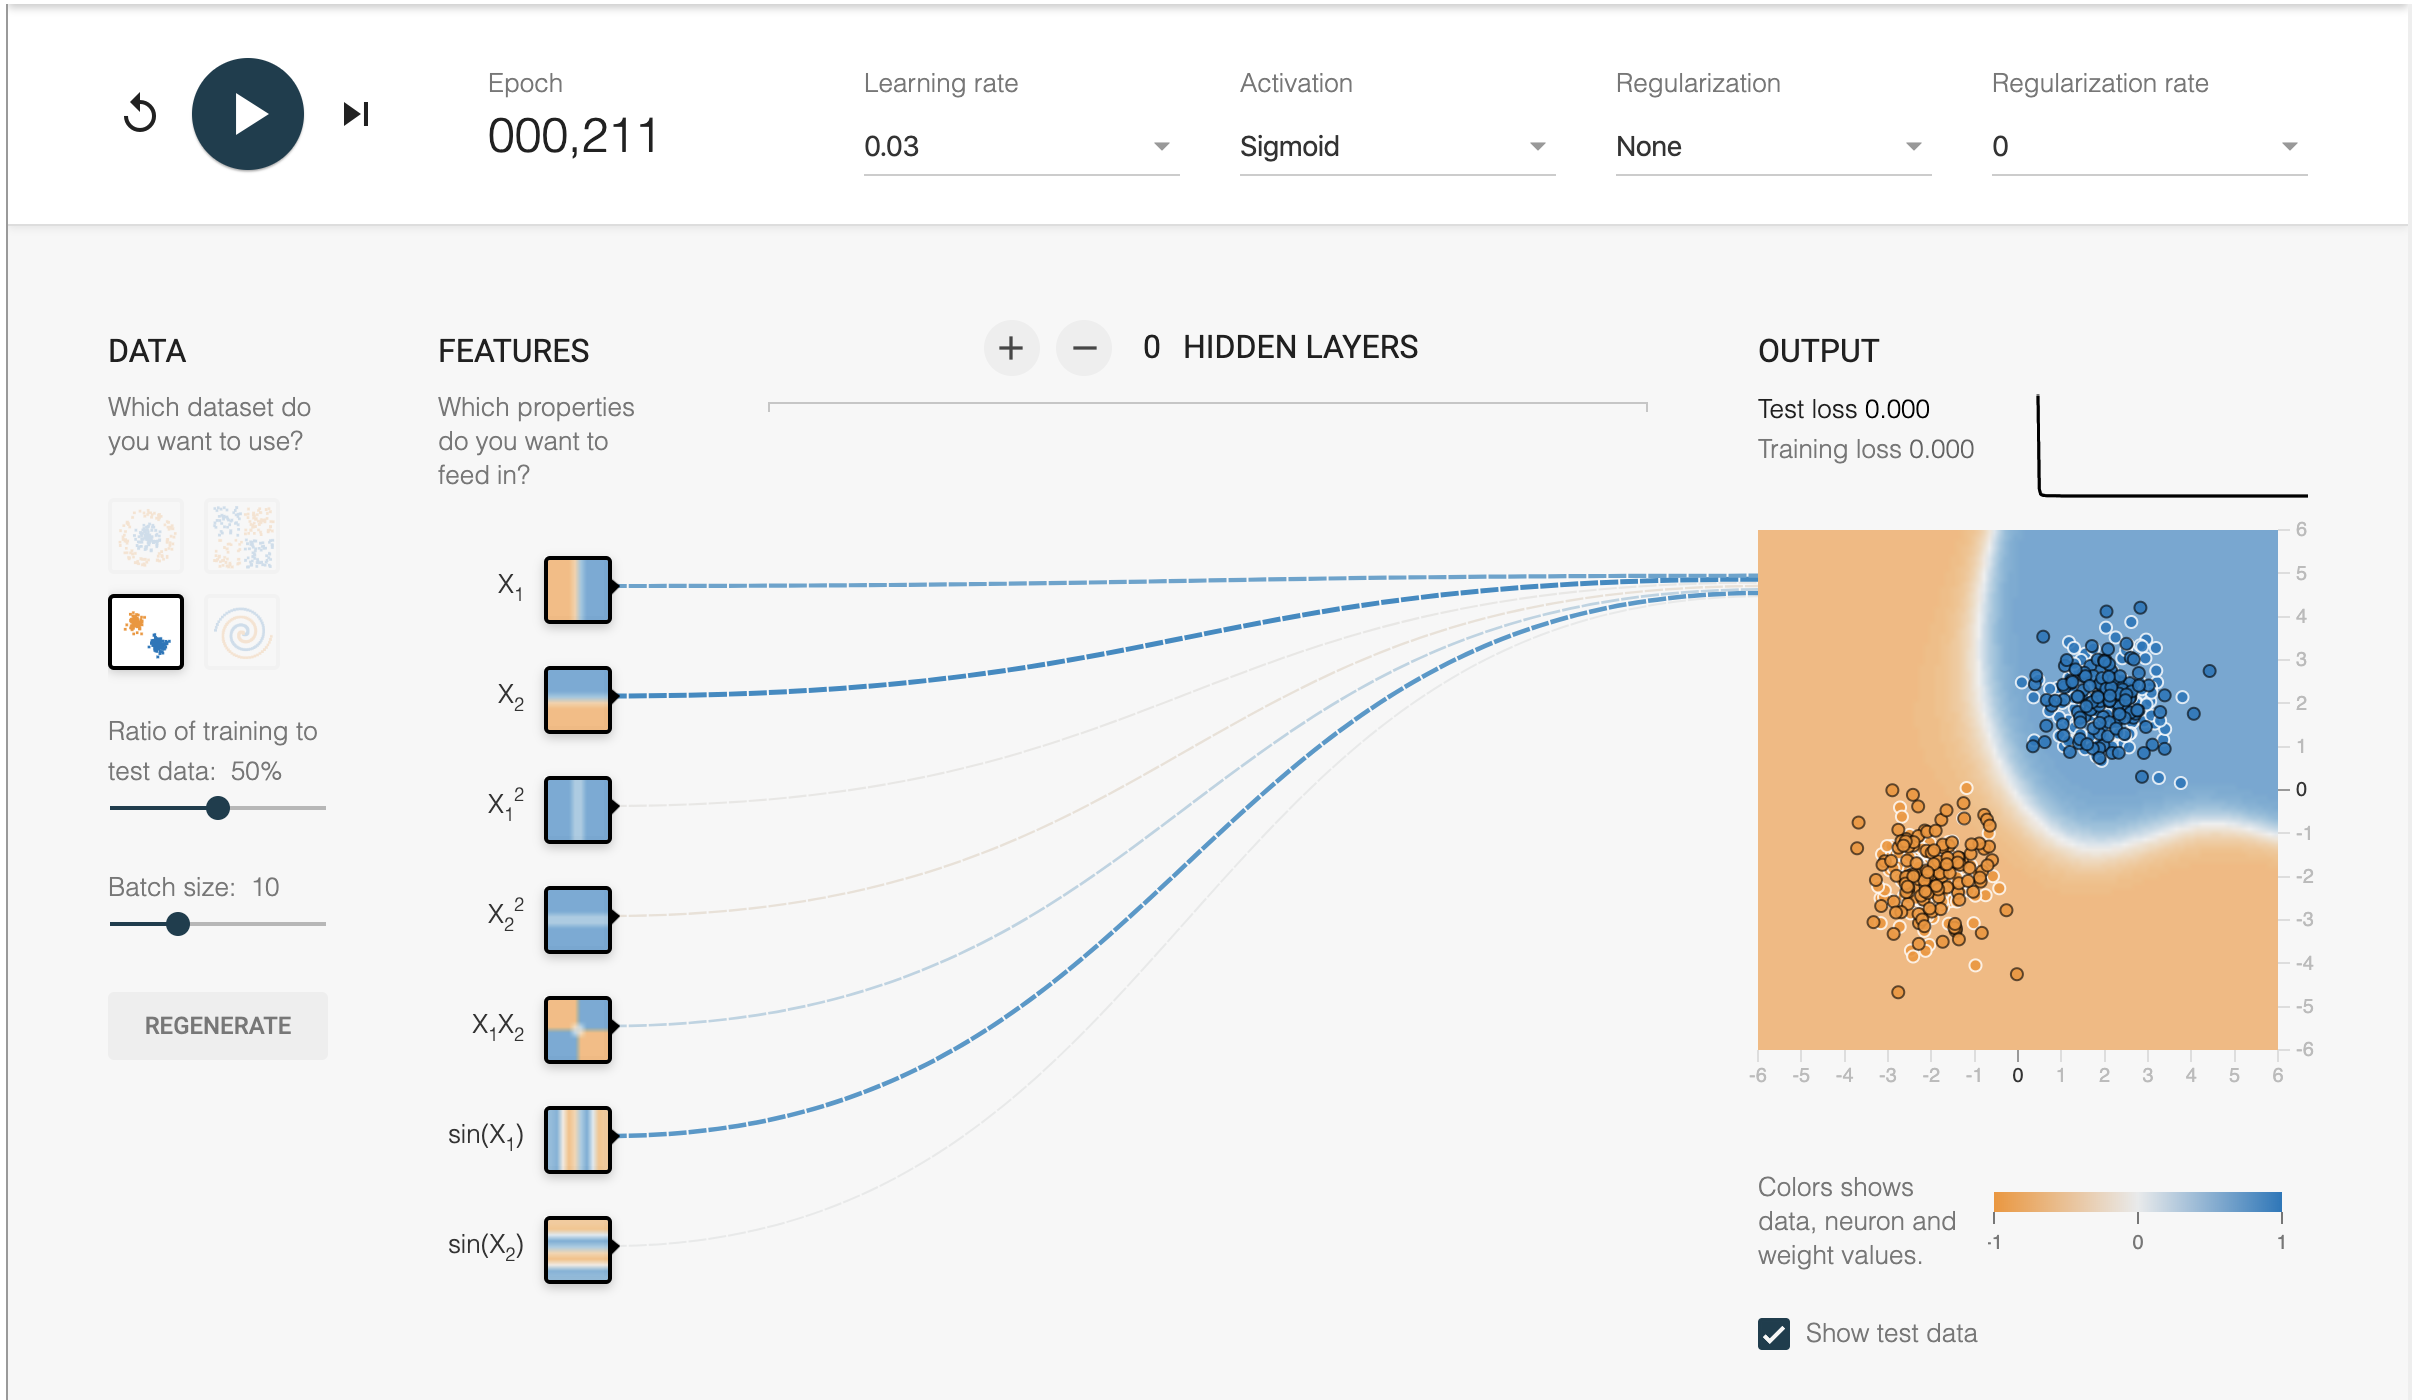
\includegraphics[width=\linewidth]{figures/1_2/gaussian.png}
  \caption{Gaussian Regularized}
  \label{fig:gaussian_reg}
\end{figure}

Task B
\medskip

The feature weights of the three models with L1 are shown in the following table.

\begin{center}
  \begin{tabular}{ |c|c|c|c|c|c|c|c| }
   \hline
     & $x_1$ & $x_2$ & $x_1^2$ & $x_2^2$ & $x_1x_2$ & $sin(x_1)$ & $sin(x_2)$ \\
    Circle & 0.0 & 0.0 & -0.38 & -0.37 & 0.0 & 0.0 & 0.0 \\
    Exclusive or & 0.0 & 0.0 & 0.0 & 0.0 & 1.7 & 0.0 & 0.0 \\
    Gaussian & 0.66 & 0.90 & -0.0034 & 0.0 & 0.0 & 0.0 & 0.0 \\
    \hline
  \end{tabular}
\end{center}

The result exactly matches the features I choose in the first question. The significant features of each data are:

\begin{center}
  \begin{tabular}{ |c|c| }
   \hline
    Circle & $x_1^2$, $x_2^2$ \\
    Exclusive or & $x_1x_2$ \\
    Gaussian & $x_1$, $x_2$ \\
    \hline
  \end{tabular}
\end{center}

1.3
\medskip

Figure \ref{fig:circle_nn} is the screenshot of circle dataset. The model structure is $8-4-2$ and the leaning rate is set to $0.1$. The testing loss descreases to $0.000$ after $1950$ iterations. It works because the three layers MLP with activation function can appromixate nonlinear boundaries like circle.

\begin{figure}[!h]
  \centering
  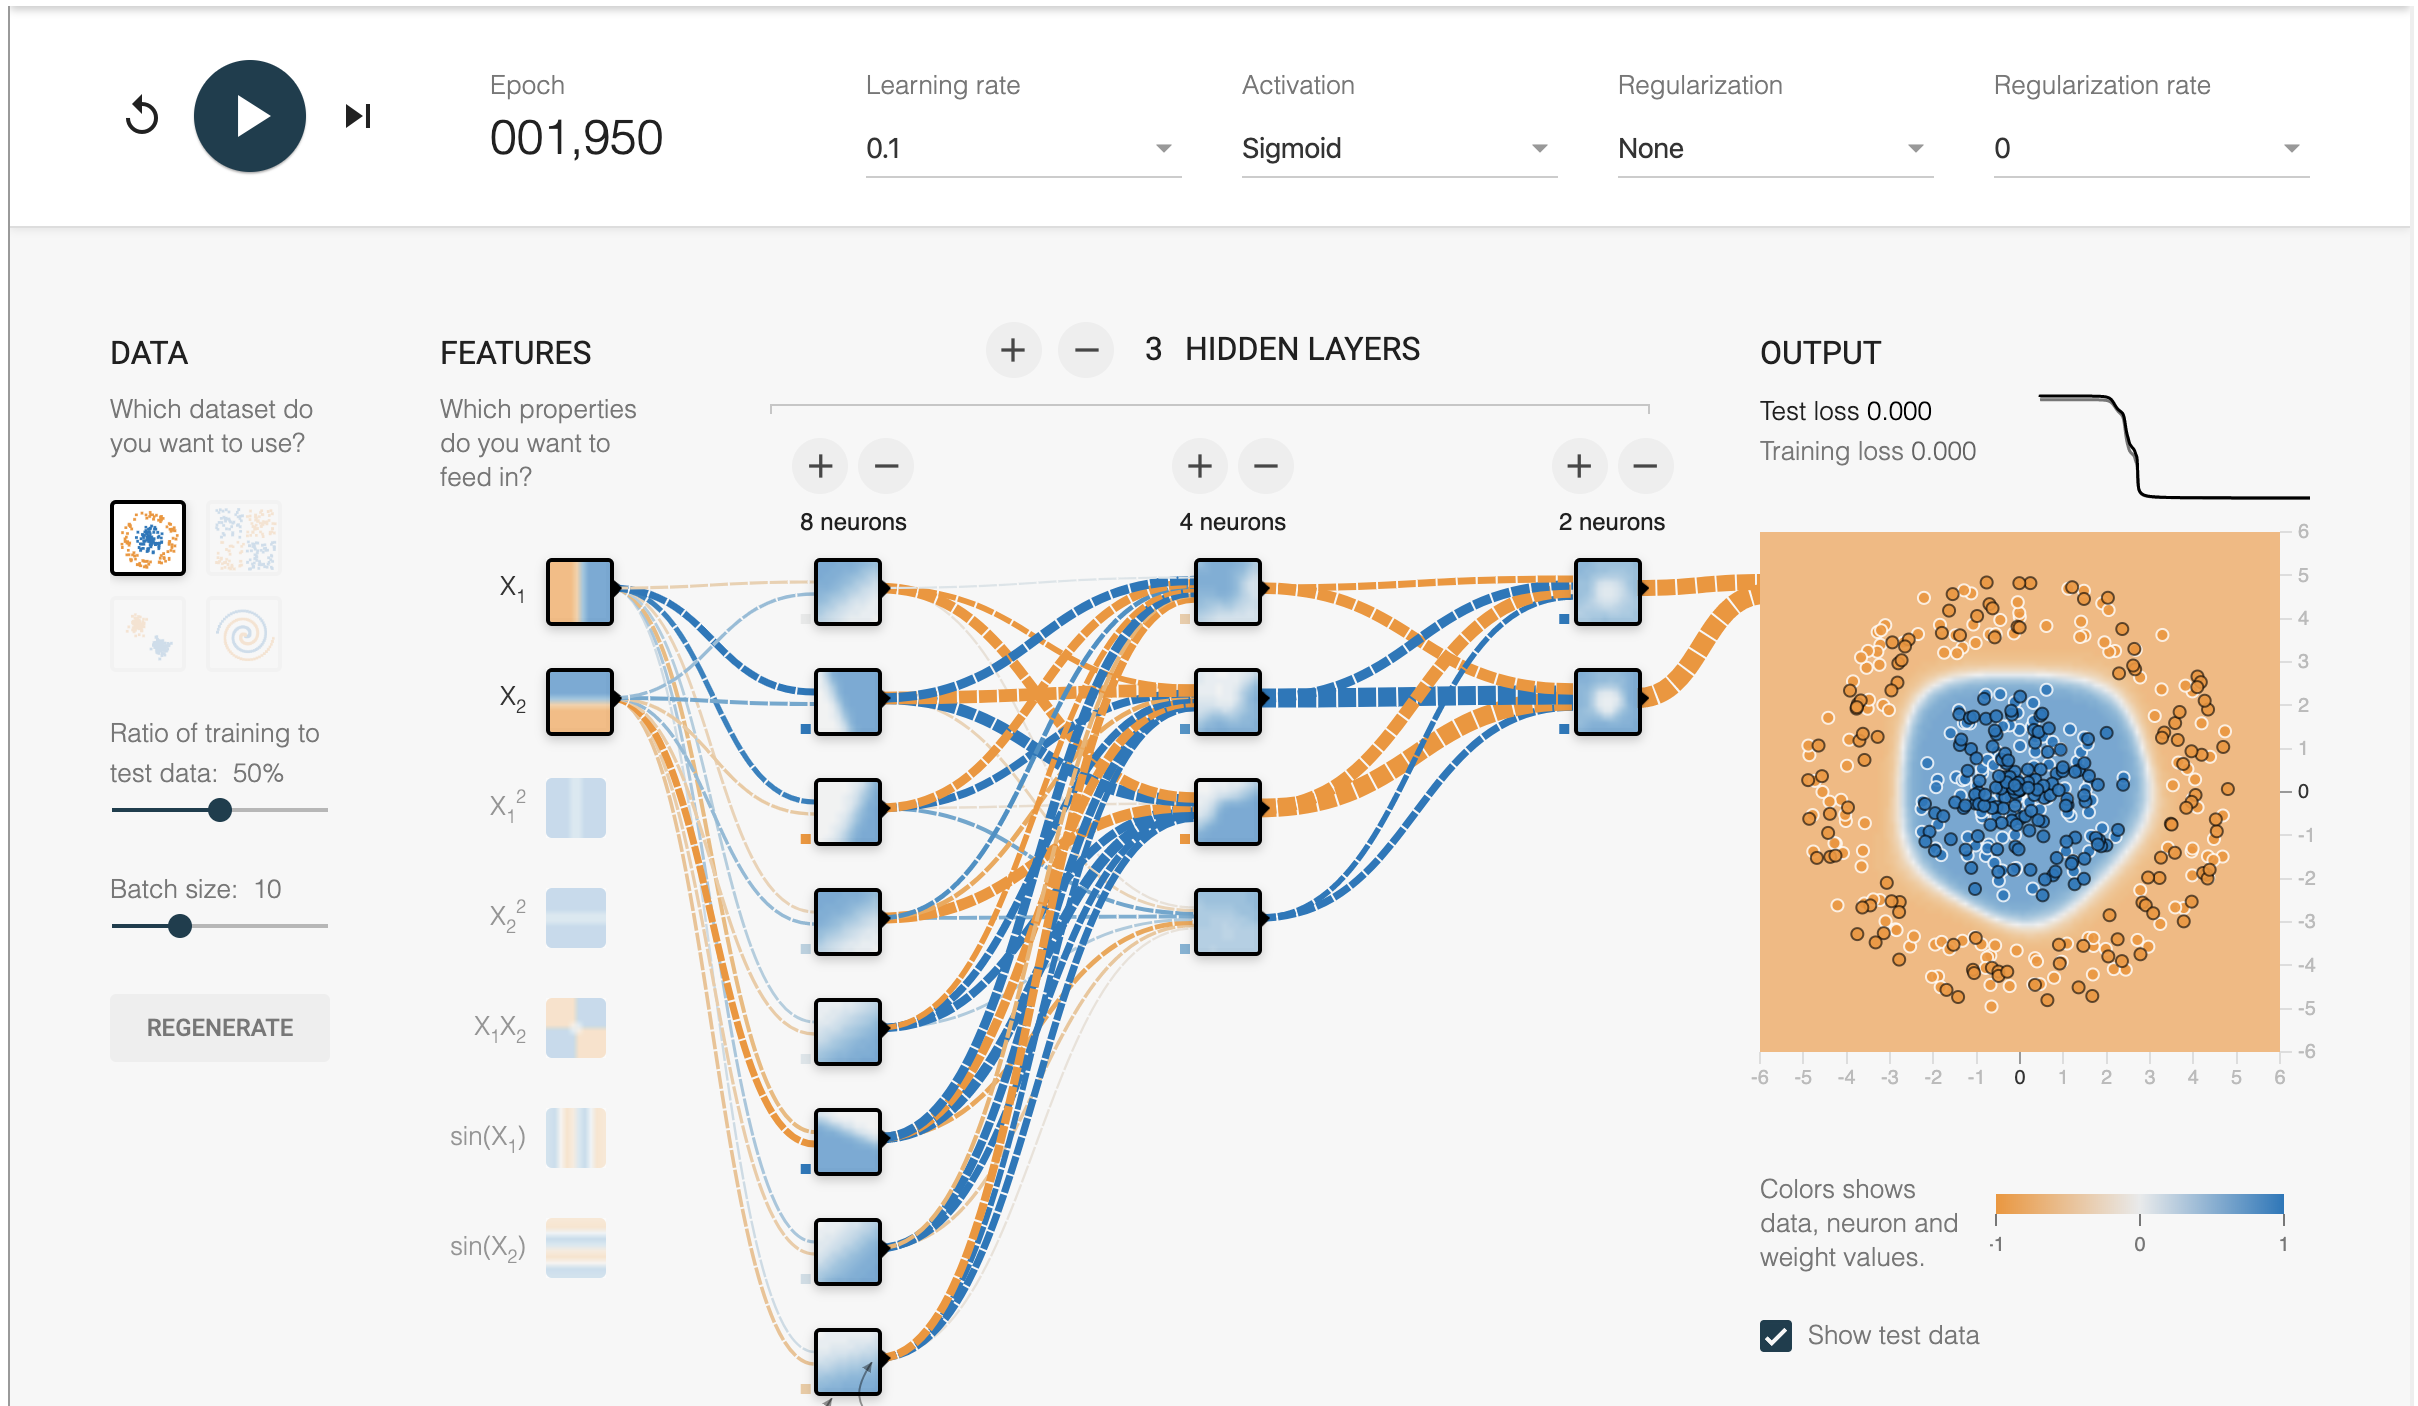
\includegraphics[width=\linewidth]{figures/1_3/circle.png}
  \caption{Circle Neural Network}
  \label{fig:circle_nn}
\end{figure}


Figure \ref{fig:exclusive_or_nn} is the screenshot of exclusive or dataset. The model structure is $8-4-2$ and the leaning rate is set to $0.1$. The testing loss descreases to $0.000$ after $803$ iterations. It works because the three layers MLP with activation function can appromixate nonlinear boundaries.

\begin{figure}[!h]
  \centering
  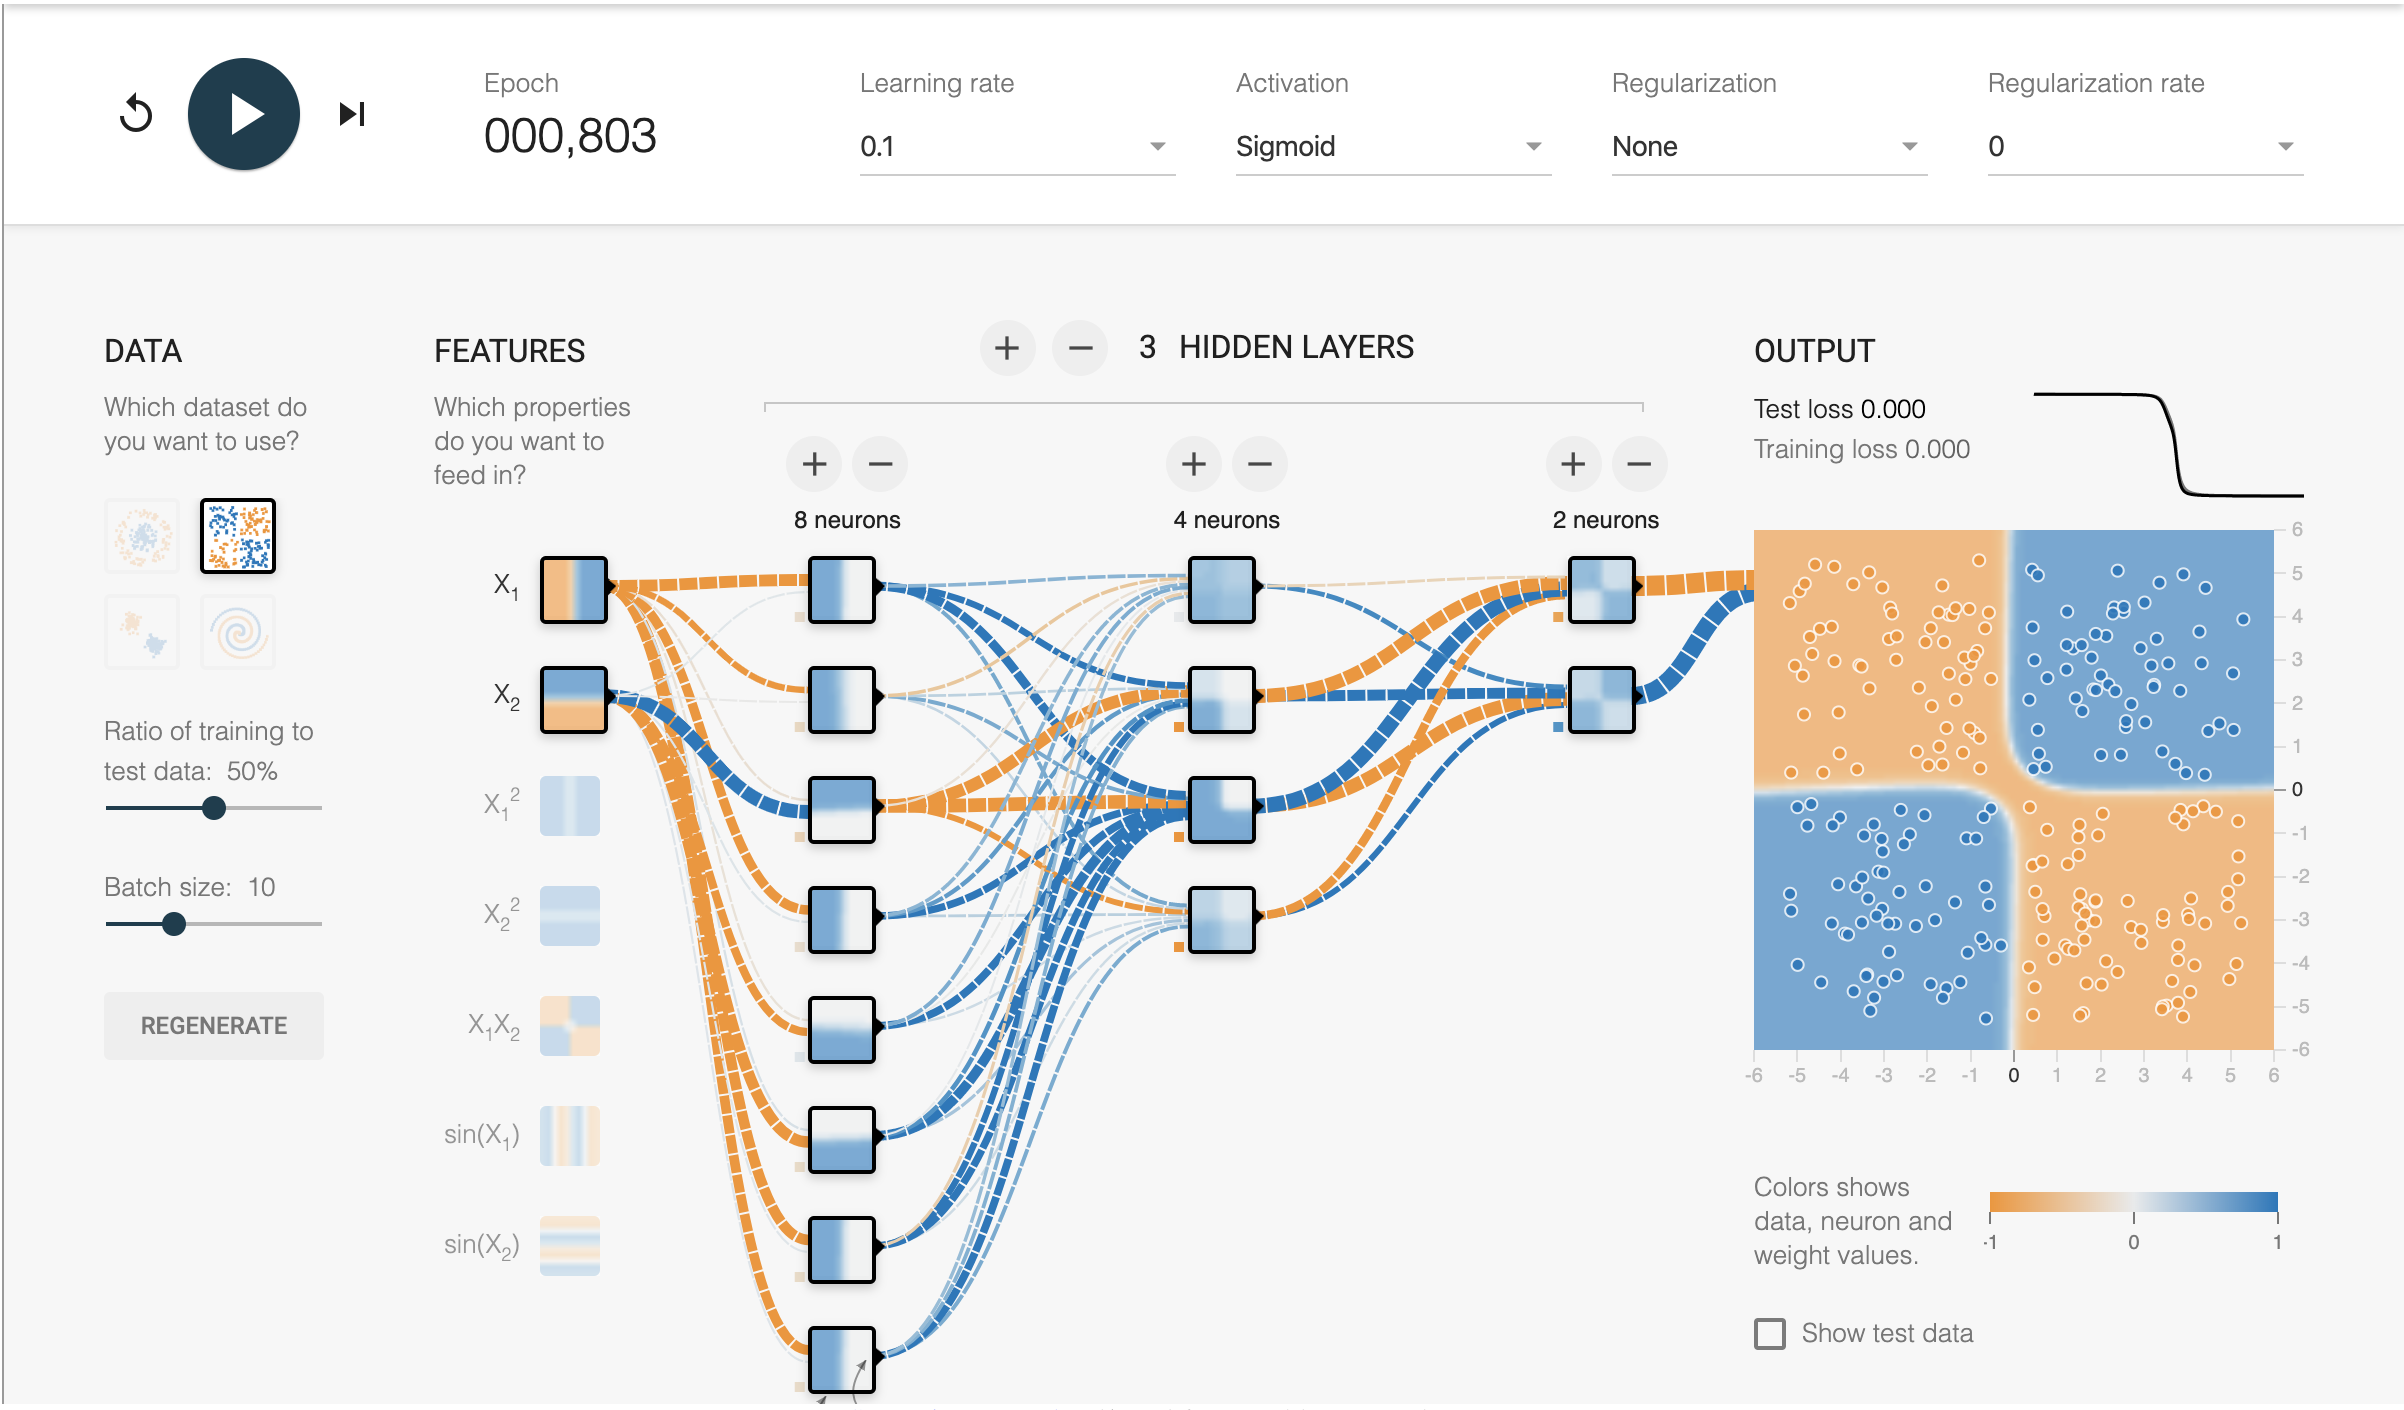
\includegraphics[width=\linewidth]{figures/1_3/exclusive_or.png}
  \caption{Exclusive Or Neural Network}
  \label{fig:exclusive_or_nn}
\end{figure}

1.4
\medskip

As shown in Firgure \ref{fig:spiral_nn}, I achieved test loss of $0.09$ on spiral dataset after $1803$ iterations (which is actually still decreasing but it will time-wasting to wait it fully converge). The model structure is simply $8-8-8-8$. It uses ReLU as the activation function and the learning rate is set to $0.03$. There is no regularization. As the screenshot shows, with 4 fully connected layers, the 4th hidden layer is able to capture those complicated spiral features, so the model works.

\begin{figure}[!h]
  \centering
  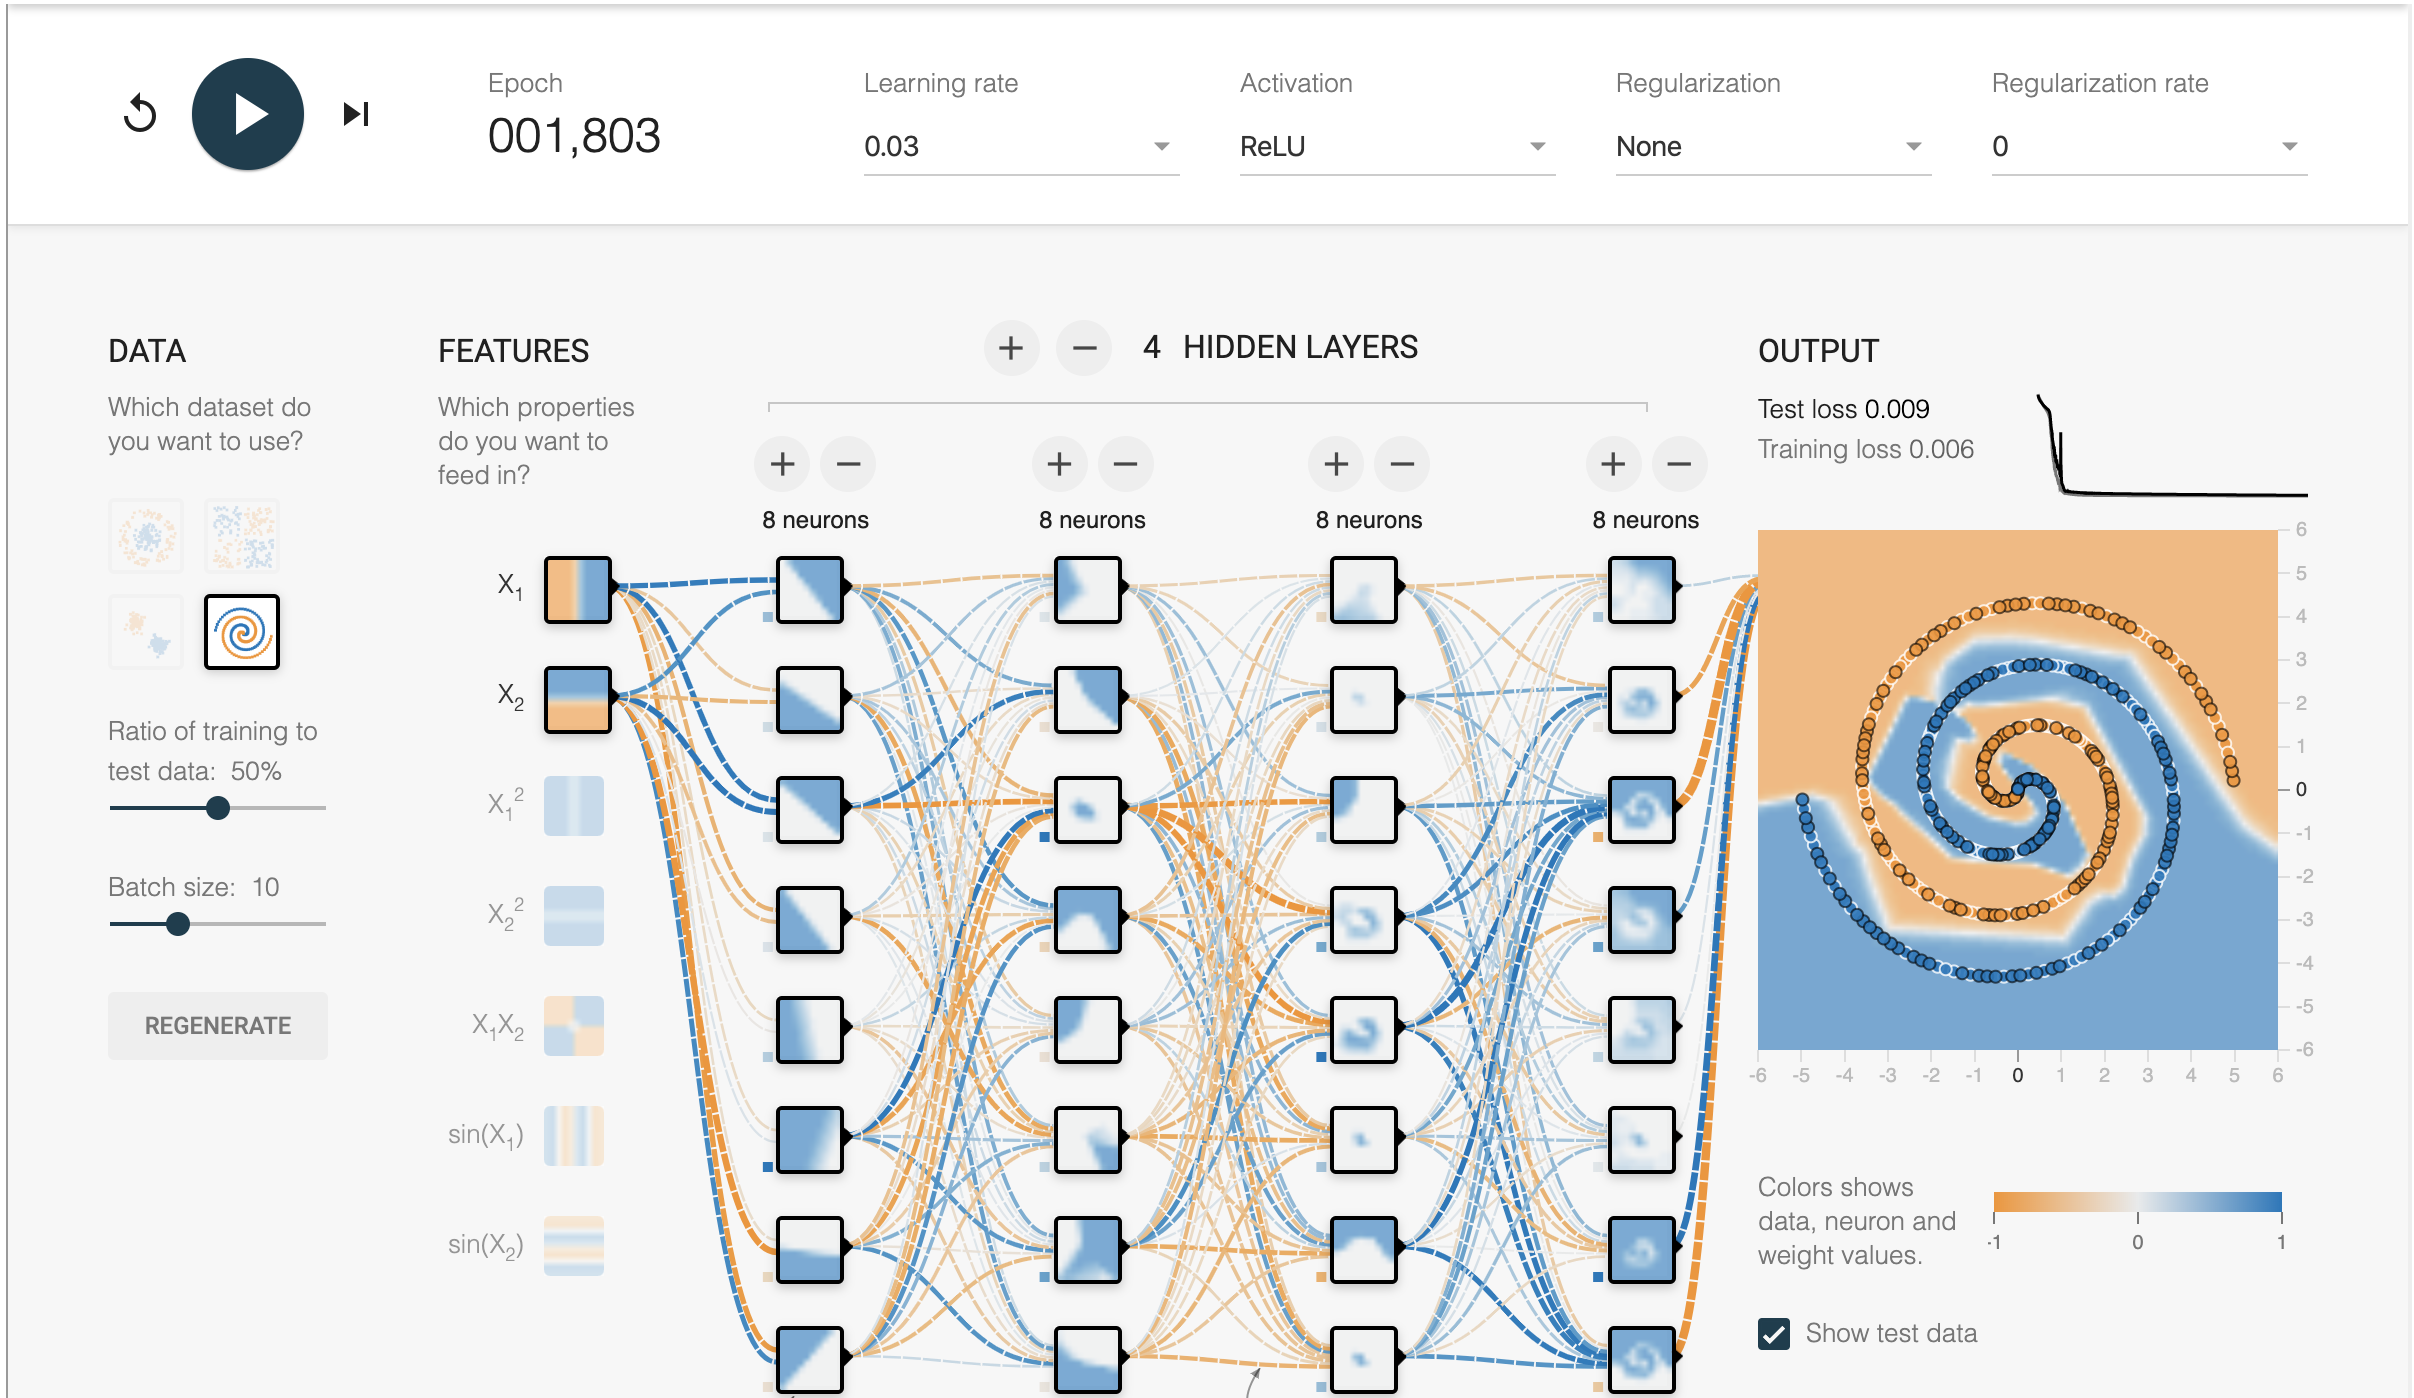
\includegraphics[width=\linewidth]{figures/1_4/spiral.png}
  \caption{Spiral Neural Network}
  \label{fig:spiral_nn}
\end{figure}

\item
Deep Learning with Keras

The 3-fold cross-validation accuracies of different hyperparameters are shown in the table below.

\item
Sample QA Questions

(a)


\medskip

(b)



% ========== Continue adding items as needed

\end{enumerate}

\end{document}
\grid
\grid
